% Generated by _scripts/md_to_tex.py from the draft; tables by _scripts/make_appendix.py.
\section{完整实验结果}\label{app:A}
本附录给出正文未展开的完整结果。附录中有两种统计口径，分别标注在各表表题中，二者不混用：与比较方法的比较（表\ref{tab:app-lifeavg}--\ref{tab:app-phase-pems08}）是三个随机种子（32、42、52）在测试集上的均值与样本标准差，种子同时决定训练初始化和节点划分，方法集合与表\ref{tab:main_speed}、表\ref{tab:main_flow}相同（四组共十一个比较方法，实现见A.5）；消融（表\ref{tab:app-abl-scenario}、表\ref{tab:app-abl-phase}）与保留节点比例实验（表\ref{tab:app-ratio}）只训练了种子32，是单次运行的结果。MAE 与 RMSE 的单位与预测变量一致，MAPE 为百分数。各表中每列最优值用红色粗体、次优值用蓝色下划线标出，按未舍入的数值排序。

\subsection{LifeAvg 结果}\label{sec:A_1}

LifeAvg 是 Unseen、Steady、Join 和 Fault 四类场景指标的等权平均。表\ref{tab:app-lifeavg}给出各方法的 LifeAvg，正文\ref{sec:4_2}节引用的总体降幅由该表的均值计算。

\begin{table}[p]
\centering
\caption{\textbf{四个数据集上的 LifeAvg 结果。}测试集，种子32、42、52的均值±样本标准差（种子同时决定节点划分）。}
\label{tab:app-lifeavg}
\small
\resizebox{\linewidth}{!}{% Generated by _scripts/make_appendix.py from frozen result files; do not edit by hand.
\begin{tabular}{lcccccc}
\toprule
方法 & \multicolumn{3}{c}{METR-LA（速度）} & \multicolumn{3}{c}{PEMS-BAY（速度）} \\
\cmidrule(lr){2-4} \cmidrule(lr){5-7}
 & MAE & RMSE & MAPE(\%) & MAE & RMSE & MAPE(\%) \\
\midrule
MoGERNN & \textcolor{blue}{\underline{4.85}}{\tiny$\pm$0.27} & \textcolor{blue}{\underline{7.06}}{\tiny$\pm$0.23} & \textcolor{blue}{\underline{13.72}}{\tiny$\pm$1.22} & \textcolor{blue}{\underline{3.19}}{\tiny$\pm$0.11} & \textcolor{blue}{\underline{4.82}}{\tiny$\pm$0.18} & \textcolor{blue}{\underline{7.95}}{\tiny$\pm$0.79} \\
SLPF & 6.26{\tiny$\pm$0.44} & 8.63{\tiny$\pm$0.50} & 19.08{\tiny$\pm$2.36} & 4.13{\tiny$\pm$0.13} & 5.88{\tiny$\pm$0.20} & 10.25{\tiny$\pm$0.62} \\
\midrule
GinAR & 10.99{\tiny$\pm$6.34} & 21.58{\tiny$\pm$19.67} & 39.22{\tiny$\pm$24.55} & 5.11{\tiny$\pm$0.38} & 7.27{\tiny$\pm$0.57} & 13.95{\tiny$\pm$1.66} \\
Merlin & 5.08{\tiny$\pm$0.12} & 7.74{\tiny$\pm$0.19} & 15.35{\tiny$\pm$1.60} & 3.31{\tiny$\pm$0.09} & 5.12{\tiny$\pm$0.17} & 8.47{\tiny$\pm$0.47} \\
\midrule
STONE & 11.01{\tiny$\pm$0.15} & 11.94{\tiny$\pm$0.17} & 26.04{\tiny$\pm$1.09} & 4.71{\tiny$\pm$0.23} & 5.86{\tiny$\pm$0.15} & 10.51{\tiny$\pm$0.11} \\
MCPST & 5.40{\tiny$\pm$0.18} & 7.65{\tiny$\pm$0.31} & 15.82{\tiny$\pm$1.19} & 3.34{\tiny$\pm$0.11} & 5.02{\tiny$\pm$0.11} & 8.32{\tiny$\pm$0.59} \\
STBP & 5.05{\tiny$\pm$0.11} & 7.73{\tiny$\pm$0.20} & 15.26{\tiny$\pm$1.67} & 3.28{\tiny$\pm$0.10} & 5.06{\tiny$\pm$0.15} & 8.32{\tiny$\pm$0.55} \\
\midrule
STGCN & 5.00{\tiny$\pm$0.05} & 7.55{\tiny$\pm$0.15} & 14.71{\tiny$\pm$0.77} & 3.24{\tiny$\pm$0.11} & 5.04{\tiny$\pm$0.17} & 8.34{\tiny$\pm$0.51} \\
STID & 5.15{\tiny$\pm$0.20} & 7.85{\tiny$\pm$0.32} & 15.85{\tiny$\pm$2.11} & 3.35{\tiny$\pm$0.14} & 5.17{\tiny$\pm$0.18} & 8.40{\tiny$\pm$0.85} \\
PatchSTG & 5.31{\tiny$\pm$0.23} & 7.90{\tiny$\pm$0.14} & 16.88{\tiny$\pm$1.02} & 3.22{\tiny$\pm$0.10} & 4.95{\tiny$\pm$0.14} & 8.02{\tiny$\pm$0.41} \\
MetaDG & 5.08{\tiny$\pm$0.30} & 7.85{\tiny$\pm$0.40} & 16.20{\tiny$\pm$1.70} & 3.48{\tiny$\pm$0.19} & 5.39{\tiny$\pm$0.21} & 9.26{\tiny$\pm$0.72} \\
\midrule
ALFNet & \textcolor{red}{\textbf{4.25}}{\tiny$\pm$0.38} & \textcolor{red}{\textbf{6.52}}{\tiny$\pm$0.44} & \textcolor{red}{\textbf{11.95}}{\tiny$\pm$1.80} & \textcolor{red}{\textbf{2.76}}{\tiny$\pm$0.08} & \textcolor{red}{\textbf{4.31}}{\tiny$\pm$0.13} & \textcolor{red}{\textbf{6.71}}{\tiny$\pm$0.41} \\
\midrule
方法 & \multicolumn{3}{c}{PEMS04（流量）} & \multicolumn{3}{c}{PEMS08（流量）} \\
\cmidrule(lr){2-4} \cmidrule(lr){5-7}
 & MAE & RMSE & MAPE(\%) & MAE & RMSE & MAPE(\%) \\
\midrule
MoGERNN & 47.05{\tiny$\pm$2.74} & 61.43{\tiny$\pm$3.26} & 43.70{\tiny$\pm$5.79} & 58.58{\tiny$\pm$0.29} & 73.42{\tiny$\pm$0.53} & 95.34{\tiny$\pm$10.08} \\
SLPF & 85.41{\tiny$\pm$9.18} & 107.71{\tiny$\pm$9.36} & 60.20{\tiny$\pm$4.06} & 90.97{\tiny$\pm$4.18} & 113.26{\tiny$\pm$4.92} & 161.13{\tiny$\pm$13.08} \\
\midrule
GinAR & 87.16{\tiny$\pm$3.44} & 109.22{\tiny$\pm$3.86} & 61.40{\tiny$\pm$3.19} & 90.60{\tiny$\pm$2.89} & 110.79{\tiny$\pm$3.07} & 146.93{\tiny$\pm$9.42} \\
Merlin & 46.11{\tiny$\pm$1.55} & 60.32{\tiny$\pm$1.54} & 34.13{\tiny$\pm$4.00} & 41.36{\tiny$\pm$0.90} & 53.39{\tiny$\pm$1.12} & 61.59{\tiny$\pm$3.82} \\
\midrule
STONE & 74.43{\tiny$\pm$2.95} & 85.73{\tiny$\pm$2.38} & 97.97{\tiny$\pm$16.01} & 63.48{\tiny$\pm$3.86} & 72.90{\tiny$\pm$4.17} & 108.47{\tiny$\pm$10.35} \\
MCPST & 45.92{\tiny$\pm$1.99} & 59.94{\tiny$\pm$2.31} & 39.84{\tiny$\pm$8.14} & 43.12{\tiny$\pm$1.62} & 54.47{\tiny$\pm$1.83} & \textcolor{blue}{\underline{59.25}}{\tiny$\pm$4.22} \\
STBP & 45.79{\tiny$\pm$1.26} & 59.78{\tiny$\pm$1.38} & 34.80{\tiny$\pm$2.64} & 42.60{\tiny$\pm$0.86} & 54.58{\tiny$\pm$1.19} & 63.72{\tiny$\pm$5.39} \\
\midrule
STGCN & \textcolor{blue}{\underline{44.49}}{\tiny$\pm$1.05} & \textcolor{blue}{\underline{58.96}}{\tiny$\pm$1.34} & 38.88{\tiny$\pm$5.47} & 45.64{\tiny$\pm$1.21} & 57.65{\tiny$\pm$1.91} & 63.66{\tiny$\pm$7.02} \\
STID & 45.51{\tiny$\pm$1.24} & 59.40{\tiny$\pm$1.10} & 35.31{\tiny$\pm$4.77} & \textcolor{blue}{\underline{41.26}}{\tiny$\pm$1.31} & \textcolor{blue}{\underline{52.96}}{\tiny$\pm$1.74} & 65.86{\tiny$\pm$2.88} \\
PatchSTG & 48.71{\tiny$\pm$1.86} & 63.64{\tiny$\pm$2.32} & 38.69{\tiny$\pm$6.11} & 45.35{\tiny$\pm$2.32} & 58.31{\tiny$\pm$2.93} & 75.86{\tiny$\pm$2.55} \\
MetaDG & 45.18{\tiny$\pm$1.62} & 59.20{\tiny$\pm$1.56} & \textcolor{blue}{\underline{33.09}}{\tiny$\pm$3.70} & 41.86{\tiny$\pm$1.91} & 53.44{\tiny$\pm$1.94} & 61.35{\tiny$\pm$7.02} \\
\midrule
ALFNet & \textcolor{red}{\textbf{37.84}}{\tiny$\pm$1.53} & \textcolor{red}{\textbf{50.70}}{\tiny$\pm$2.33} & \textcolor{red}{\textbf{26.88}}{\tiny$\pm$3.86} & \textcolor{red}{\textbf{38.95}}{\tiny$\pm$2.08} & \textcolor{red}{\textbf{49.28}}{\tiny$\pm$2.39} & \textcolor{red}{\textbf{48.37}}{\tiny$\pm$6.43} \\
\bottomrule
\end{tabular}
}
\end{table}

\subsection{分阶段完整结果}\label{sec:A_2}

表\ref{tab:app-phase-metrla}--\ref{tab:app-phase-pems08}给出各方法在 Join 的 Cold、Warm、Ready 阶段和 Fault 的 Onset、Decay、Outage 阶段的全部指标，是正文图\ref{fig:condition}的数据来源。

\begin{table}[p]
\centering
\caption{\textbf{METR-LA 的分阶段结果。}测试集，种子32、42、52的均值±样本标准差。上半部分为 Join 的三个阶段，下半部分为 Fault 的三个阶段。}
\label{tab:app-phase-metrla}
\small
\resizebox{\linewidth}{!}{% Generated by _scripts/make_appendix.py from frozen result files; do not edit by hand.
\begin{tabular}{lccccccccc}
\toprule
方法 & \multicolumn{3}{c}{Join: Cold} & \multicolumn{3}{c}{Join: Warm} & \multicolumn{3}{c}{Join: Ready} \\
\cmidrule(lr){2-4} \cmidrule(lr){5-7} \cmidrule(lr){8-10}
 & MAE & RMSE & MAPE(\%) & MAE & RMSE & MAPE(\%) & MAE & RMSE & MAPE(\%) \\
\midrule
MoGERNN & 4.84{\tiny$\pm$0.45} & \textcolor{blue}{\underline{7.09}}{\tiny$\pm$0.54} & 14.04{\tiny$\pm$2.68} & 4.70{\tiny$\pm$0.48} & 6.99{\tiny$\pm$0.55} & 13.74{\tiny$\pm$2.21} & 4.44{\tiny$\pm$0.34} & 6.69{\tiny$\pm$0.56} & 12.10{\tiny$\pm$2.48} \\
SLPF & 6.70{\tiny$\pm$0.30} & 9.07{\tiny$\pm$0.48} & 19.20{\tiny$\pm$3.38} & 6.74{\tiny$\pm$0.21} & 9.06{\tiny$\pm$0.44} & 19.68{\tiny$\pm$2.97} & 6.11{\tiny$\pm$0.30} & 8.32{\tiny$\pm$0.60} & 16.47{\tiny$\pm$2.20} \\
\midrule
GinAR & 7.97{\tiny$\pm$0.49} & 10.91{\tiny$\pm$0.68} & 26.27{\tiny$\pm$7.45} & 8.46{\tiny$\pm$0.36} & 11.47{\tiny$\pm$0.56} & 28.23{\tiny$\pm$4.86} & 7.81{\tiny$\pm$0.01} & 10.70{\tiny$\pm$0.42} & 24.11{\tiny$\pm$3.19} \\
Merlin & \textcolor{blue}{\underline{4.64}}{\tiny$\pm$0.12} & 7.19{\tiny$\pm$0.39} & \textcolor{blue}{\underline{13.04}}{\tiny$\pm$1.48} & 4.25{\tiny$\pm$0.24} & \textcolor{blue}{\underline{6.91}}{\tiny$\pm$0.46} & \textcolor{blue}{\underline{12.12}}{\tiny$\pm$1.57} & 3.99{\tiny$\pm$0.30} & 6.58{\tiny$\pm$0.59} & \textcolor{blue}{\underline{10.93}}{\tiny$\pm$2.01} \\
\midrule
STONE & 10.60{\tiny$\pm$0.05} & 11.56{\tiny$\pm$0.14} & 24.64{\tiny$\pm$2.40} & 10.61{\tiny$\pm$0.41} & 11.46{\tiny$\pm$0.49} & 25.02{\tiny$\pm$2.48} & 10.30{\tiny$\pm$0.22} & 11.12{\tiny$\pm$0.27} & 22.61{\tiny$\pm$1.40} \\
MCPST & 5.05{\tiny$\pm$0.29} & 7.31{\tiny$\pm$0.59} & 15.58{\tiny$\pm$3.42} & 4.57{\tiny$\pm$0.36} & 7.00{\tiny$\pm$0.55} & 13.58{\tiny$\pm$2.07} & 4.27{\tiny$\pm$0.25} & 6.62{\tiny$\pm$0.50} & 11.75{\tiny$\pm$1.63} \\
STBP & 4.87{\tiny$\pm$0.03} & 7.40{\tiny$\pm$0.26} & 13.64{\tiny$\pm$1.40} & 4.37{\tiny$\pm$0.08} & 6.99{\tiny$\pm$0.27} & 12.79{\tiny$\pm$1.42} & 4.00{\tiny$\pm$0.19} & 6.55{\tiny$\pm$0.41} & 11.23{\tiny$\pm$1.52} \\
\midrule
STGCN & 5.19{\tiny$\pm$0.12} & 7.62{\tiny$\pm$0.20} & 14.47{\tiny$\pm$0.90} & 4.53{\tiny$\pm$0.38} & 7.14{\tiny$\pm$0.58} & 13.29{\tiny$\pm$1.86} & 4.20{\tiny$\pm$0.37} & 6.75{\tiny$\pm$0.65} & 11.92{\tiny$\pm$1.90} \\
STID & 5.01{\tiny$\pm$0.26} & 7.58{\tiny$\pm$0.46} & 13.86{\tiny$\pm$0.74} & 4.45{\tiny$\pm$0.12} & 7.11{\tiny$\pm$0.30} & 12.71{\tiny$\pm$1.30} & 4.08{\tiny$\pm$0.11} & 6.64{\tiny$\pm$0.33} & 11.03{\tiny$\pm$1.56} \\
PatchSTG & 5.37{\tiny$\pm$0.37} & 7.68{\tiny$\pm$0.73} & 15.95{\tiny$\pm$1.66} & 4.59{\tiny$\pm$0.55} & 7.17{\tiny$\pm$0.77} & 13.69{\tiny$\pm$1.68} & 4.27{\tiny$\pm$0.25} & 6.78{\tiny$\pm$0.54} & 12.11{\tiny$\pm$1.23} \\
MetaDG & 5.10{\tiny$\pm$0.75} & 7.74{\tiny$\pm$0.94} & 14.90{\tiny$\pm$3.87} & \textcolor{blue}{\underline{4.20}}{\tiny$\pm$0.38} & 6.92{\tiny$\pm$0.55} & 12.80{\tiny$\pm$2.13} & \textcolor{blue}{\underline{3.88}}{\tiny$\pm$0.27} & \textcolor{blue}{\underline{6.51}}{\tiny$\pm$0.55} & 11.26{\tiny$\pm$2.31} \\
\midrule
ALFNet & \textcolor{red}{\textbf{4.39}}{\tiny$\pm$0.62} & \textcolor{red}{\textbf{6.50}}{\tiny$\pm$0.79} & \textcolor{red}{\textbf{12.24}}{\tiny$\pm$3.09} & \textcolor{red}{\textbf{3.96}}{\tiny$\pm$0.51} & \textcolor{red}{\textbf{6.33}}{\tiny$\pm$0.70} & \textcolor{red}{\textbf{11.61}}{\tiny$\pm$2.63} & \textcolor{red}{\textbf{3.62}}{\tiny$\pm$0.44} & \textcolor{red}{\textbf{5.98}}{\tiny$\pm$0.81} & \textcolor{red}{\textbf{10.28}}{\tiny$\pm$2.77} \\
\midrule
方法 & \multicolumn{3}{c}{Fault: Onset} & \multicolumn{3}{c}{Fault: Decay} & \multicolumn{3}{c}{Fault: Outage} \\
\cmidrule(lr){2-4} \cmidrule(lr){5-7} \cmidrule(lr){8-10}
 & MAE & RMSE & MAPE(\%) & MAE & RMSE & MAPE(\%) & MAE & RMSE & MAPE(\%) \\
\midrule
MoGERNN & 4.25{\tiny$\pm$0.23} & 6.36{\tiny$\pm$0.23} & 12.49{\tiny$\pm$1.03} & 4.51{\tiny$\pm$0.11} & \textcolor{blue}{\underline{6.65}}{\tiny$\pm$0.08} & \textcolor{blue}{\underline{13.04}}{\tiny$\pm$0.45} & 5.39{\tiny$\pm$0.27} & \textcolor{blue}{\underline{7.61}}{\tiny$\pm$0.32} & \textcolor{blue}{\underline{16.25}}{\tiny$\pm$1.40} \\
SLPF & 5.74{\tiny$\pm$1.21} & 8.20{\tiny$\pm$1.42} & 19.13{\tiny$\pm$5.87} & 5.70{\tiny$\pm$1.10} & 8.13{\tiny$\pm$1.28} & 18.52{\tiny$\pm$3.70} & 6.28{\tiny$\pm$1.11} & 8.84{\tiny$\pm$1.31} & 21.80{\tiny$\pm$5.31} \\
\midrule
GinAR & 6.50{\tiny$\pm$0.27} & 9.41{\tiny$\pm$0.32} & 22.26{\tiny$\pm$1.88} & 6.24{\tiny$\pm$0.57} & 9.14{\tiny$\pm$0.68} & 21.60{\tiny$\pm$2.10} & 6.73{\tiny$\pm$0.76} & 9.87{\tiny$\pm$0.95} & 24.61{\tiny$\pm$1.75} \\
Merlin & 4.01{\tiny$\pm$0.26} & 6.40{\tiny$\pm$0.36} & \textcolor{blue}{\underline{11.24}}{\tiny$\pm$0.63} & 4.46{\tiny$\pm$0.37} & 6.96{\tiny$\pm$0.39} & 13.73{\tiny$\pm$1.09} & 5.74{\tiny$\pm$1.11} & 8.47{\tiny$\pm$1.20} & 20.23{\tiny$\pm$5.54} \\
\midrule
STONE & 10.49{\tiny$\pm$0.50} & 11.33{\tiny$\pm$0.60} & 24.86{\tiny$\pm$3.70} & 10.65{\tiny$\pm$0.19} & 11.51{\tiny$\pm$0.20} & 24.90{\tiny$\pm$0.97} & 11.32{\tiny$\pm$0.60} & 12.34{\tiny$\pm$0.63} & 28.41{\tiny$\pm$3.06} \\
MCPST & 5.06{\tiny$\pm$0.27} & 7.20{\tiny$\pm$0.27} & 16.05{\tiny$\pm$2.73} & 5.36{\tiny$\pm$0.06} & 7.62{\tiny$\pm$0.03} & 15.96{\tiny$\pm$0.37} & 7.80{\tiny$\pm$0.11} & 10.28{\tiny$\pm$0.08} & 25.40{\tiny$\pm$1.87} \\
STBP & \textcolor{blue}{\underline{3.95}}{\tiny$\pm$0.23} & \textcolor{blue}{\underline{6.27}}{\tiny$\pm$0.33} & 11.85{\tiny$\pm$0.89} & \textcolor{blue}{\underline{4.30}}{\tiny$\pm$0.21} & 6.80{\tiny$\pm$0.29} & 13.16{\tiny$\pm$0.81} & 5.21{\tiny$\pm$0.36} & 8.15{\tiny$\pm$0.43} & 17.74{\tiny$\pm$1.55} \\
\midrule
STGCN & 4.07{\tiny$\pm$0.07} & 6.53{\tiny$\pm$0.10} & 11.90{\tiny$\pm$1.18} & 4.44{\tiny$\pm$0.08} & 6.93{\tiny$\pm$0.10} & 13.79{\tiny$\pm$0.19} & \textcolor{blue}{\underline{5.04}}{\tiny$\pm$0.17} & 7.78{\tiny$\pm$0.27} & 16.61{\tiny$\pm$1.01} \\
STID & 4.25{\tiny$\pm$0.30} & 6.69{\tiny$\pm$0.38} & 13.38{\tiny$\pm$1.38} & 4.54{\tiny$\pm$0.45} & 7.15{\tiny$\pm$0.59} & 14.61{\tiny$\pm$2.03} & 5.63{\tiny$\pm$1.13} & 8.67{\tiny$\pm$1.48} & 20.29{\tiny$\pm$5.56} \\
PatchSTG & 4.81{\tiny$\pm$0.48} & 7.31{\tiny$\pm$0.34} & 15.50{\tiny$\pm$1.03} & 5.02{\tiny$\pm$0.97} & 7.64{\tiny$\pm$1.09} & 16.82{\tiny$\pm$4.42} & 6.32{\tiny$\pm$2.25} & 9.25{\tiny$\pm$2.52} & 22.90{\tiny$\pm$8.80} \\
MetaDG & 4.11{\tiny$\pm$0.15} & 6.57{\tiny$\pm$0.25} & 12.55{\tiny$\pm$0.84} & 4.60{\tiny$\pm$0.09} & 7.27{\tiny$\pm$0.06} & 14.66{\tiny$\pm$0.40} & 6.74{\tiny$\pm$0.71} & 9.97{\tiny$\pm$0.79} & 25.00{\tiny$\pm$3.31} \\
\midrule
ALFNet & \textcolor{red}{\textbf{3.68}}{\tiny$\pm$0.20} & \textcolor{red}{\textbf{5.88}}{\tiny$\pm$0.36} & \textcolor{red}{\textbf{10.76}}{\tiny$\pm$0.83} & \textcolor{red}{\textbf{3.81}}{\tiny$\pm$0.22} & \textcolor{red}{\textbf{6.04}}{\tiny$\pm$0.28} & \textcolor{red}{\textbf{11.14}}{\tiny$\pm$0.87} & \textcolor{red}{\textbf{4.20}}{\tiny$\pm$0.27} & \textcolor{red}{\textbf{6.57}}{\tiny$\pm$0.39} & \textcolor{red}{\textbf{12.64}}{\tiny$\pm$0.95} \\
\bottomrule
\end{tabular}
}
\end{table}

\begin{table}[p]
\centering
\caption{\textbf{PEMS-BAY 的分阶段结果。}记号与表\ref{tab:app-phase-metrla}相同。}
\label{tab:app-phase-pemsbay}
\small
\resizebox{\linewidth}{!}{% Generated by _scripts/make_appendix.py from frozen result files; do not edit by hand.
\begin{tabular}{lccccccccc}
\toprule
方法 & \multicolumn{3}{c}{Join: Cold} & \multicolumn{3}{c}{Join: Warm} & \multicolumn{3}{c}{Join: Ready} \\
\cmidrule(lr){2-4} \cmidrule(lr){5-7} \cmidrule(lr){8-10}
 & MAE & RMSE & MAPE(\%) & MAE & RMSE & MAPE(\%) & MAE & RMSE & MAPE(\%) \\
\midrule
MoGERNN & 2.91{\tiny$\pm$0.16} & 4.50{\tiny$\pm$0.20} & 7.17{\tiny$\pm$0.63} & 2.75{\tiny$\pm$0.15} & 4.40{\tiny$\pm$0.18} & 6.89{\tiny$\pm$0.90} & 2.73{\tiny$\pm$0.16} & 4.32{\tiny$\pm$0.21} & 6.63{\tiny$\pm$0.86} \\
SLPF & 4.60{\tiny$\pm$0.09} & 6.37{\tiny$\pm$0.19} & 10.79{\tiny$\pm$0.09} & 4.64{\tiny$\pm$0.18} & 6.48{\tiny$\pm$0.31} & 11.01{\tiny$\pm$0.89} & 4.60{\tiny$\pm$0.09} & 6.41{\tiny$\pm$0.25} & 11.01{\tiny$\pm$0.48} \\
\midrule
GinAR & 6.00{\tiny$\pm$0.36} & 8.27{\tiny$\pm$0.54} & 16.22{\tiny$\pm$1.61} & 6.23{\tiny$\pm$0.52} & 8.58{\tiny$\pm$0.79} & 16.78{\tiny$\pm$2.40} & 6.20{\tiny$\pm$0.34} & 8.57{\tiny$\pm$0.61} & 16.75{\tiny$\pm$1.41} \\
Merlin & \textcolor{blue}{\underline{2.51}}{\tiny$\pm$0.13} & \textcolor{blue}{\underline{4.09}}{\tiny$\pm$0.23} & \textcolor{red}{\textbf{5.88}}{\tiny$\pm$0.47} & \textcolor{blue}{\underline{2.45}}{\tiny$\pm$0.09} & \textcolor{blue}{\underline{4.11}}{\tiny$\pm$0.18} & 5.93{\tiny$\pm$0.40} & \textcolor{blue}{\underline{2.37}}{\tiny$\pm$0.07} & \textcolor{blue}{\underline{4.00}}{\tiny$\pm$0.17} & \textcolor{blue}{\underline{5.66}}{\tiny$\pm$0.25} \\
\midrule
STONE & 4.30{\tiny$\pm$0.30} & 5.28{\tiny$\pm$0.24} & 9.15{\tiny$\pm$0.61} & 4.22{\tiny$\pm$0.22} & 5.22{\tiny$\pm$0.10} & 9.05{\tiny$\pm$0.23} & 4.22{\tiny$\pm$0.24} & 5.19{\tiny$\pm$0.12} & 9.00{\tiny$\pm$0.51} \\
MCPST & 3.00{\tiny$\pm$0.02} & 4.48{\tiny$\pm$0.08} & 7.15{\tiny$\pm$0.38} & 2.71{\tiny$\pm$0.02} & 4.40{\tiny$\pm$0.05} & 6.46{\tiny$\pm$0.36} & 2.60{\tiny$\pm$0.04} & 4.29{\tiny$\pm$0.07} & 6.21{\tiny$\pm$0.16} \\
STBP & 2.71{\tiny$\pm$0.13} & 4.36{\tiny$\pm$0.28} & 6.47{\tiny$\pm$0.65} & 2.50{\tiny$\pm$0.08} & 4.19{\tiny$\pm$0.15} & \textcolor{blue}{\underline{5.85}}{\tiny$\pm$0.10} & 2.40{\tiny$\pm$0.02} & 4.05{\tiny$\pm$0.09} & \textcolor{red}{\textbf{5.51}}{\tiny$\pm$0.14} \\
\midrule
STGCN & 2.87{\tiny$\pm$0.06} & 4.41{\tiny$\pm$0.17} & 7.16{\tiny$\pm$0.17} & 2.49{\tiny$\pm$0.04} & 4.23{\tiny$\pm$0.10} & 6.19{\tiny$\pm$0.27} & 2.42{\tiny$\pm$0.05} & 4.15{\tiny$\pm$0.13} & 5.92{\tiny$\pm$0.44} \\
STID & 2.84{\tiny$\pm$0.05} & 4.54{\tiny$\pm$0.15} & 6.68{\tiny$\pm$0.15} & 2.61{\tiny$\pm$0.06} & 4.34{\tiny$\pm$0.15} & 6.03{\tiny$\pm$0.24} & 2.51{\tiny$\pm$0.04} & 4.21{\tiny$\pm$0.13} & 5.71{\tiny$\pm$0.23} \\
PatchSTG & 3.02{\tiny$\pm$0.03} & 4.74{\tiny$\pm$0.14} & 7.19{\tiny$\pm$0.23} & 2.73{\tiny$\pm$0.13} & 4.48{\tiny$\pm$0.25} & 6.43{\tiny$\pm$0.57} & 2.55{\tiny$\pm$0.14} & 4.24{\tiny$\pm$0.35} & 6.00{\tiny$\pm$0.54} \\
MetaDG & 3.26{\tiny$\pm$0.19} & 4.93{\tiny$\pm$0.31} & 7.75{\tiny$\pm$0.44} & 2.58{\tiny$\pm$0.11} & 4.30{\tiny$\pm$0.11} & 6.20{\tiny$\pm$0.52} & 2.45{\tiny$\pm$0.16} & 4.17{\tiny$\pm$0.22} & 5.89{\tiny$\pm$0.63} \\
\midrule
ALFNet & \textcolor{red}{\textbf{2.45}}{\tiny$\pm$0.07} & \textcolor{red}{\textbf{3.92}}{\tiny$\pm$0.20} & \textcolor{blue}{\underline{5.91}}{\tiny$\pm$0.26} & \textcolor{red}{\textbf{2.35}}{\tiny$\pm$0.06} & \textcolor{red}{\textbf{3.95}}{\tiny$\pm$0.12} & \textcolor{red}{\textbf{5.81}}{\tiny$\pm$0.38} & \textcolor{red}{\textbf{2.30}}{\tiny$\pm$0.08} & \textcolor{red}{\textbf{3.87}}{\tiny$\pm$0.22} & 5.67{\tiny$\pm$0.44} \\
\midrule
方法 & \multicolumn{3}{c}{Fault: Onset} & \multicolumn{3}{c}{Fault: Decay} & \multicolumn{3}{c}{Fault: Outage} \\
\cmidrule(lr){2-4} \cmidrule(lr){5-7} \cmidrule(lr){8-10}
 & MAE & RMSE & MAPE(\%) & MAE & RMSE & MAPE(\%) & MAE & RMSE & MAPE(\%) \\
\midrule
MoGERNN & 2.54{\tiny$\pm$0.15} & 3.96{\tiny$\pm$0.22} & 6.59{\tiny$\pm$0.61} & 2.93{\tiny$\pm$0.13} & 4.53{\tiny$\pm$0.25} & 7.57{\tiny$\pm$1.00} & 4.20{\tiny$\pm$0.13} & 5.98{\tiny$\pm$0.24} & 10.31{\tiny$\pm$0.44} \\
SLPF & 3.35{\tiny$\pm$0.14} & 4.84{\tiny$\pm$0.17} & 8.40{\tiny$\pm$0.87} & 3.44{\tiny$\pm$0.09} & 5.06{\tiny$\pm$0.14} & 8.74{\tiny$\pm$0.57} & 3.75{\tiny$\pm$0.06} & 5.55{\tiny$\pm$0.14} & 9.86{\tiny$\pm$0.34} \\
\midrule
GinAR & 3.92{\tiny$\pm$0.03} & 5.84{\tiny$\pm$0.00} & 10.88{\tiny$\pm$0.81} & 4.02{\tiny$\pm$0.39} & 5.99{\tiny$\pm$0.53} & 11.15{\tiny$\pm$1.72} & 4.18{\tiny$\pm$0.11} & 6.30{\tiny$\pm$0.21} & 11.67{\tiny$\pm$0.20} \\
Merlin & 2.15{\tiny$\pm$0.11} & 3.53{\tiny$\pm$0.17} & 5.27{\tiny$\pm$0.60} & 2.65{\tiny$\pm$0.18} & 4.26{\tiny$\pm$0.26} & 6.78{\tiny$\pm$0.76} & 3.36{\tiny$\pm$0.12} & 5.34{\tiny$\pm$0.10} & 8.87{\tiny$\pm$0.37} \\
\midrule
STONE & 4.13{\tiny$\pm$0.43} & 4.93{\tiny$\pm$0.37} & 8.33{\tiny$\pm$0.78} & 4.40{\tiny$\pm$0.36} & 5.38{\tiny$\pm$0.33} & 9.15{\tiny$\pm$0.50} & 4.69{\tiny$\pm$0.48} & 6.10{\tiny$\pm$0.52} & 10.58{\tiny$\pm$1.20} \\
MCPST & 3.02{\tiny$\pm$0.21} & 4.63{\tiny$\pm$0.28} & 8.68{\tiny$\pm$1.13} & 3.31{\tiny$\pm$0.08} & 4.91{\tiny$\pm$0.09} & 8.32{\tiny$\pm$0.54} & 4.71{\tiny$\pm$0.26} & 6.56{\tiny$\pm$0.32} & 11.79{\tiny$\pm$0.71} \\
STBP & 2.33{\tiny$\pm$0.24} & 3.74{\tiny$\pm$0.33} & 6.16{\tiny$\pm$1.25} & 2.63{\tiny$\pm$0.14} & 4.20{\tiny$\pm$0.23} & 6.69{\tiny$\pm$0.39} & 3.67{\tiny$\pm$0.54} & 5.63{\tiny$\pm$0.67} & 10.03{\tiny$\pm$2.37} \\
\midrule
STGCN & 2.26{\tiny$\pm$0.16} & 3.75{\tiny$\pm$0.19} & 5.62{\tiny$\pm$0.78} & 2.98{\tiny$\pm$0.05} & 4.73{\tiny$\pm$0.12} & 7.87{\tiny$\pm$0.30} & 4.30{\tiny$\pm$0.16} & 6.48{\tiny$\pm$0.30} & 11.54{\tiny$\pm$0.60} \\
STID & 2.35{\tiny$\pm$0.07} & 3.81{\tiny$\pm$0.08} & 5.53{\tiny$\pm$0.71} & 2.69{\tiny$\pm$0.14} & 4.31{\tiny$\pm$0.23} & 6.78{\tiny$\pm$0.68} & 3.36{\tiny$\pm$0.11} & 5.33{\tiny$\pm$0.19} & 8.98{\tiny$\pm$0.54} \\
PatchSTG & \textcolor{blue}{\underline{2.09}}{\tiny$\pm$0.17} & \textcolor{blue}{\underline{3.39}}{\tiny$\pm$0.23} & \textcolor{blue}{\underline{5.10}}{\tiny$\pm$0.92} & \textcolor{blue}{\underline{2.35}}{\tiny$\pm$0.06} & \textcolor{blue}{\underline{3.84}}{\tiny$\pm$0.08} & \textcolor{blue}{\underline{5.79}}{\tiny$\pm$0.26} & \textcolor{red}{\textbf{2.75}}{\tiny$\pm$0.10} & \textcolor{blue}{\underline{4.52}}{\tiny$\pm$0.11} & \textcolor{blue}{\underline{6.88}}{\tiny$\pm$0.36} \\
MetaDG & 2.20{\tiny$\pm$0.15} & 3.64{\tiny$\pm$0.13} & 5.26{\tiny$\pm$0.89} & 2.80{\tiny$\pm$0.13} & 4.55{\tiny$\pm$0.16} & 7.18{\tiny$\pm$0.53} & 4.67{\tiny$\pm$0.08} & 6.96{\tiny$\pm$0.04} & 13.46{\tiny$\pm$0.64} \\
\midrule
ALFNet & \textcolor{red}{\textbf{1.93}}{\tiny$\pm$0.09} & \textcolor{red}{\textbf{3.15}}{\tiny$\pm$0.17} & \textcolor{red}{\textbf{4.52}}{\tiny$\pm$0.53} & \textcolor{red}{\textbf{2.23}}{\tiny$\pm$0.05} & \textcolor{red}{\textbf{3.62}}{\tiny$\pm$0.10} & \textcolor{red}{\textbf{5.40}}{\tiny$\pm$0.30} & \textcolor{blue}{\underline{2.85}}{\tiny$\pm$0.06} & \textcolor{red}{\textbf{4.42}}{\tiny$\pm$0.08} & \textcolor{red}{\textbf{6.74}}{\tiny$\pm$0.08} \\
\bottomrule
\end{tabular}
}
\end{table}

\begin{table}[p]
\centering
\caption{\textbf{PEMS04 的分阶段结果。}记号与表\ref{tab:app-phase-metrla}相同。}
\label{tab:app-phase-pems04}
\small
\resizebox{\linewidth}{!}{% Generated by _scripts/make_appendix.py from frozen result files; do not edit by hand.
\begin{tabular}{lccccccccc}
\toprule
方法 & \multicolumn{3}{c}{Join: Cold} & \multicolumn{3}{c}{Join: Warm} & \multicolumn{3}{c}{Join: Ready} \\
\cmidrule(lr){2-4} \cmidrule(lr){5-7} \cmidrule(lr){8-10}
 & MAE & RMSE & MAPE(\%) & MAE & RMSE & MAPE(\%) & MAE & RMSE & MAPE(\%) \\
\midrule
MoGERNN & 54.36{\tiny$\pm$4.43} & 71.30{\tiny$\pm$5.26} & 52.94{\tiny$\pm$14.97} & 46.52{\tiny$\pm$4.27} & 61.31{\tiny$\pm$5.34} & 41.99{\tiny$\pm$5.07} & 43.01{\tiny$\pm$3.66} & 57.06{\tiny$\pm$4.56} & 35.81{\tiny$\pm$3.93} \\
SLPF & 90.49{\tiny$\pm$9.58} & 112.75{\tiny$\pm$10.21} & 61.05{\tiny$\pm$3.97} & 87.76{\tiny$\pm$11.62} & 109.39{\tiny$\pm$11.82} & 62.77{\tiny$\pm$4.41} & 84.27{\tiny$\pm$11.88} & 105.95{\tiny$\pm$12.65} & 66.11{\tiny$\pm$8.75} \\
\midrule
GinAR & 93.82{\tiny$\pm$4.46} & 116.58{\tiny$\pm$6.03} & 65.97{\tiny$\pm$8.13} & 91.76{\tiny$\pm$6.07} & 113.93{\tiny$\pm$6.76} & 67.31{\tiny$\pm$7.15} & 88.20{\tiny$\pm$6.83} & 110.49{\tiny$\pm$8.10} & 69.13{\tiny$\pm$10.13} \\
Merlin & \textcolor{blue}{\underline{31.00}}{\tiny$\pm$0.29} & \textcolor{blue}{\underline{44.86}}{\tiny$\pm$0.62} & \textcolor{blue}{\underline{23.22}}{\tiny$\pm$5.22} & 26.20{\tiny$\pm$0.55} & 37.71{\tiny$\pm$0.90} & 19.77{\tiny$\pm$3.39} & 26.10{\tiny$\pm$1.19} & 36.94{\tiny$\pm$1.82} & 20.22{\tiny$\pm$3.41} \\
\midrule
STONE & 66.07{\tiny$\pm$3.10} & 76.20{\tiny$\pm$3.57} & 99.98{\tiny$\pm$27.22} & 63.47{\tiny$\pm$0.87} & 71.69{\tiny$\pm$0.83} & 94.02{\tiny$\pm$21.85} & 64.04{\tiny$\pm$5.02} & 72.61{\tiny$\pm$4.59} & 90.23{\tiny$\pm$22.43} \\
MCPST & 39.33{\tiny$\pm$1.43} & 53.44{\tiny$\pm$1.78} & 40.91{\tiny$\pm$14.92} & 30.81{\tiny$\pm$0.96} & 42.51{\tiny$\pm$1.25} & 26.23{\tiny$\pm$5.37} & 29.26{\tiny$\pm$1.48} & 40.56{\tiny$\pm$1.58} & 25.14{\tiny$\pm$4.60} \\
STBP & 31.80{\tiny$\pm$0.71} & 45.58{\tiny$\pm$1.27} & 23.98{\tiny$\pm$5.43} & 26.62{\tiny$\pm$0.74} & 37.88{\tiny$\pm$1.37} & 21.75{\tiny$\pm$3.55} & 25.94{\tiny$\pm$0.93} & 36.51{\tiny$\pm$1.50} & 22.06{\tiny$\pm$3.65} \\
\midrule
STGCN & 42.17{\tiny$\pm$2.19} & 55.90{\tiny$\pm$2.84} & 33.75{\tiny$\pm$7.75} & 30.87{\tiny$\pm$1.39} & 42.28{\tiny$\pm$1.92} & 24.82{\tiny$\pm$2.41} & 28.46{\tiny$\pm$1.86} & 39.44{\tiny$\pm$2.33} & 22.82{\tiny$\pm$2.20} \\
STID & 32.82{\tiny$\pm$0.29} & 46.85{\tiny$\pm$0.38} & 25.44{\tiny$\pm$6.05} & \textcolor{blue}{\underline{25.99}}{\tiny$\pm$0.25} & \textcolor{blue}{\underline{37.53}}{\tiny$\pm$0.52} & 21.53{\tiny$\pm$4.68} & 25.34{\tiny$\pm$0.97} & 36.15{\tiny$\pm$1.72} & 20.43{\tiny$\pm$4.17} \\
PatchSTG & 46.15{\tiny$\pm$10.64} & 63.28{\tiny$\pm$12.31} & 34.81{\tiny$\pm$14.47} & 35.07{\tiny$\pm$6.18} & 50.17{\tiny$\pm$8.26} & 30.02{\tiny$\pm$8.18} & 32.67{\tiny$\pm$6.27} & 46.35{\tiny$\pm$8.63} & 30.15{\tiny$\pm$8.04} \\
MetaDG & 39.65{\tiny$\pm$1.34} & 56.94{\tiny$\pm$2.50} & 27.93{\tiny$\pm$5.11} & 26.97{\tiny$\pm$1.02} & 38.92{\tiny$\pm$1.57} & \textcolor{blue}{\underline{19.49}}{\tiny$\pm$2.34} & \textcolor{blue}{\underline{25.17}}{\tiny$\pm$1.57} & \textcolor{blue}{\underline{36.02}}{\tiny$\pm$2.13} & \textcolor{blue}{\underline{18.13}}{\tiny$\pm$1.45} \\
\midrule
ALFNet & \textcolor{red}{\textbf{29.82}}{\tiny$\pm$1.03} & \textcolor{red}{\textbf{41.93}}{\tiny$\pm$1.46} & \textcolor{red}{\textbf{22.33}}{\tiny$\pm$6.29} & \textcolor{red}{\textbf{25.11}}{\tiny$\pm$0.77} & \textcolor{red}{\textbf{35.70}}{\tiny$\pm$1.53} & \textcolor{red}{\textbf{17.73}}{\tiny$\pm$2.79} & \textcolor{red}{\textbf{24.83}}{\tiny$\pm$1.24} & \textcolor{red}{\textbf{34.95}}{\tiny$\pm$1.84} & \textcolor{red}{\textbf{17.03}}{\tiny$\pm$2.54} \\
\midrule
方法 & \multicolumn{3}{c}{Fault: Onset} & \multicolumn{3}{c}{Fault: Decay} & \multicolumn{3}{c}{Fault: Outage} \\
\cmidrule(lr){2-4} \cmidrule(lr){5-7} \cmidrule(lr){8-10}
 & MAE & RMSE & MAPE(\%) & MAE & RMSE & MAPE(\%) & MAE & RMSE & MAPE(\%) \\
\midrule
MoGERNN & 34.42{\tiny$\pm$2.27} & 45.34{\tiny$\pm$2.89} & 26.98{\tiny$\pm$7.58} & 37.77{\tiny$\pm$1.39} & 48.97{\tiny$\pm$1.57} & 33.49{\tiny$\pm$4.96} & 51.21{\tiny$\pm$2.14} & 67.04{\tiny$\pm$2.33} & 48.25{\tiny$\pm$3.13} \\
SLPF & 85.45{\tiny$\pm$8.60} & 108.25{\tiny$\pm$8.22} & 55.39{\tiny$\pm$10.51} & 83.09{\tiny$\pm$7.83} & 106.04{\tiny$\pm$7.70} & 55.22{\tiny$\pm$6.27} & 83.22{\tiny$\pm$5.59} & 105.36{\tiny$\pm$6.04} & 60.83{\tiny$\pm$7.11} \\
\midrule
GinAR & 85.20{\tiny$\pm$2.03} & 107.34{\tiny$\pm$1.80} & 53.55{\tiny$\pm$4.76} & 82.56{\tiny$\pm$1.46} & 104.29{\tiny$\pm$1.64} & 53.86{\tiny$\pm$1.95} & 82.41{\tiny$\pm$3.29} & 103.23{\tiny$\pm$4.77} & 58.29{\tiny$\pm$0.14} \\
Merlin & 27.93{\tiny$\pm$0.75} & 39.05{\tiny$\pm$1.23} & 17.76{\tiny$\pm$1.32} & 32.44{\tiny$\pm$0.69} & 44.19{\tiny$\pm$0.89} & 21.39{\tiny$\pm$0.45} & 86.47{\tiny$\pm$2.19} & 108.77{\tiny$\pm$3.13} & 62.31{\tiny$\pm$5.46} \\
\midrule
STONE & 62.71{\tiny$\pm$5.48} & 71.38{\tiny$\pm$5.00} & 72.16{\tiny$\pm$20.34} & 64.10{\tiny$\pm$3.96} & 73.92{\tiny$\pm$2.99} & 89.63{\tiny$\pm$15.43} & 98.75{\tiny$\pm$1.77} & 117.42{\tiny$\pm$2.25} & 124.91{\tiny$\pm$7.99} \\
MCPST & 32.86{\tiny$\pm$1.73} & 44.15{\tiny$\pm$2.27} & 27.43{\tiny$\pm$2.55} & 40.72{\tiny$\pm$1.30} & 53.38{\tiny$\pm$1.61} & 32.30{\tiny$\pm$0.97} & 79.06{\tiny$\pm$2.06} & 100.70{\tiny$\pm$3.33} & 64.45{\tiny$\pm$6.31} \\
STBP & 27.65{\tiny$\pm$0.32} & 38.17{\tiny$\pm$0.34} & 18.27{\tiny$\pm$1.58} & 32.81{\tiny$\pm$0.55} & 44.28{\tiny$\pm$0.66} & 22.77{\tiny$\pm$0.71} & 87.70{\tiny$\pm$2.19} & 109.45{\tiny$\pm$2.76} & 63.74{\tiny$\pm$4.34} \\
\midrule
STGCN & 29.23{\tiny$\pm$0.68} & 40.03{\tiny$\pm$0.84} & 18.84{\tiny$\pm$0.94} & 38.08{\tiny$\pm$0.74} & 50.56{\tiny$\pm$0.94} & 28.86{\tiny$\pm$0.86} & 76.69{\tiny$\pm$5.35} & 101.83{\tiny$\pm$6.27} & 78.34{\tiny$\pm$3.20} \\
STID & 26.66{\tiny$\pm$0.53} & 37.22{\tiny$\pm$0.89} & 16.38{\tiny$\pm$0.83} & 33.49{\tiny$\pm$0.83} & 45.17{\tiny$\pm$0.78} & 23.26{\tiny$\pm$1.75} & 86.11{\tiny$\pm$2.53} & 107.63{\tiny$\pm$2.52} & 65.60{\tiny$\pm$5.83} \\
PatchSTG & 27.56{\tiny$\pm$2.62} & 37.62{\tiny$\pm$3.74} & 20.72{\tiny$\pm$3.89} & 30.97{\tiny$\pm$3.27} & \textcolor{blue}{\underline{41.72}}{\tiny$\pm$4.21} & 22.47{\tiny$\pm$2.35} & \textcolor{blue}{\underline{46.27}}{\tiny$\pm$16.60} & \textcolor{blue}{\underline{62.39}}{\tiny$\pm$21.19} & \textcolor{red}{\textbf{34.49}}{\tiny$\pm$11.66} \\
MetaDG & \textcolor{blue}{\underline{26.00}}{\tiny$\pm$0.73} & \textcolor{blue}{\underline{36.47}}{\tiny$\pm$1.14} & \textcolor{blue}{\underline{15.40}}{\tiny$\pm$0.75} & \textcolor{blue}{\underline{30.54}}{\tiny$\pm$0.13} & 41.76{\tiny$\pm$0.30} & \textcolor{blue}{\underline{18.82}}{\tiny$\pm$0.28} & 87.08{\tiny$\pm$2.25} & 108.95{\tiny$\pm$2.12} & 63.50{\tiny$\pm$3.83} \\
\midrule
ALFNet & \textcolor{red}{\textbf{24.81}}{\tiny$\pm$0.62} & \textcolor{red}{\textbf{34.73}}{\tiny$\pm$0.83} & \textcolor{red}{\textbf{14.93}}{\tiny$\pm$0.84} & \textcolor{red}{\textbf{29.19}}{\tiny$\pm$0.11} & \textcolor{red}{\textbf{39.67}}{\tiny$\pm$0.28} & \textcolor{red}{\textbf{18.62}}{\tiny$\pm$0.53} & \textcolor{red}{\textbf{44.92}}{\tiny$\pm$3.14} & \textcolor{red}{\textbf{59.41}}{\tiny$\pm$5.19} & \textcolor{blue}{\underline{35.71}}{\tiny$\pm$1.27} \\
\bottomrule
\end{tabular}
}
\end{table}

\begin{table}[p]
\centering
\caption{\textbf{PEMS08 的分阶段结果。}记号与表\ref{tab:app-phase-metrla}相同。}
\label{tab:app-phase-pems08}
\small
\resizebox{\linewidth}{!}{% Generated by _scripts/make_appendix.py from frozen result files; do not edit by hand.
\begin{tabular}{lccccccccc}
\toprule
方法 & \multicolumn{3}{c}{Join: Cold} & \multicolumn{3}{c}{Join: Warm} & \multicolumn{3}{c}{Join: Ready} \\
\cmidrule(lr){2-4} \cmidrule(lr){5-7} \cmidrule(lr){8-10}
 & MAE & RMSE & MAPE(\%) & MAE & RMSE & MAPE(\%) & MAE & RMSE & MAPE(\%) \\
\midrule
MoGERNN & 70.42{\tiny$\pm$4.20} & 86.25{\tiny$\pm$5.33} & 143.37{\tiny$\pm$24.11} & 69.60{\tiny$\pm$2.05} & 85.70{\tiny$\pm$3.00} & 141.69{\tiny$\pm$23.17} & 67.77{\tiny$\pm$6.86} & 82.69{\tiny$\pm$8.46} & 122.02{\tiny$\pm$6.53} \\
SLPF & 97.30{\tiny$\pm$12.19} & 121.89{\tiny$\pm$15.24} & 211.27{\tiny$\pm$19.05} & 100.32{\tiny$\pm$9.39} & 125.97{\tiny$\pm$11.10} & 232.18{\tiny$\pm$24.35} & 107.02{\tiny$\pm$11.67} & 132.93{\tiny$\pm$15.03} & 253.24{\tiny$\pm$50.15} \\
\midrule
GinAR & 93.80{\tiny$\pm$3.23} & 113.84{\tiny$\pm$4.21} & 178.00{\tiny$\pm$27.07} & 97.31{\tiny$\pm$4.69} & 118.76{\tiny$\pm$5.52} & 193.23{\tiny$\pm$30.82} & 103.54{\tiny$\pm$3.68} & 126.05{\tiny$\pm$4.52} & 207.26{\tiny$\pm$38.13} \\
Merlin & \textcolor{blue}{\underline{21.52}}{\tiny$\pm$2.58} & \textcolor{blue}{\underline{29.98}}{\tiny$\pm$3.30} & \textcolor{blue}{\underline{36.09}}{\tiny$\pm$4.44} & 20.91{\tiny$\pm$2.12} & 29.41{\tiny$\pm$2.98} & \textcolor{blue}{\underline{22.29}}{\tiny$\pm$3.22} & 22.69{\tiny$\pm$3.08} & 32.24{\tiny$\pm$4.65} & 21.54{\tiny$\pm$1.96} \\
\midrule
STONE & 55.08{\tiny$\pm$2.03} & 62.15{\tiny$\pm$2.00} & 107.86{\tiny$\pm$7.24} & 53.09{\tiny$\pm$3.25} & 58.91{\tiny$\pm$2.95} & 93.39{\tiny$\pm$14.59} & 52.35{\tiny$\pm$1.92} & 58.24{\tiny$\pm$1.48} & 88.44{\tiny$\pm$24.80} \\
MCPST & 32.70{\tiny$\pm$3.63} & 40.83{\tiny$\pm$4.10} & 68.04{\tiny$\pm$3.00} & 26.04{\tiny$\pm$2.68} & 34.39{\tiny$\pm$3.27} & 31.11{\tiny$\pm$0.84} & 26.38{\tiny$\pm$2.99} & 35.24{\tiny$\pm$3.28} & 27.65{\tiny$\pm$4.03} \\
STBP & 24.72{\tiny$\pm$1.11} & 33.37{\tiny$\pm$1.82} & 42.10{\tiny$\pm$13.70} & 21.94{\tiny$\pm$1.31} & 30.28{\tiny$\pm$1.64} & 28.57{\tiny$\pm$3.30} & 21.89{\tiny$\pm$1.66} & 30.60{\tiny$\pm$2.02} & 25.09{\tiny$\pm$4.27} \\
\midrule
STGCN & 43.47{\tiny$\pm$3.35} & 54.74{\tiny$\pm$3.85} & 90.54{\tiny$\pm$18.51} & 30.27{\tiny$\pm$2.08} & 39.32{\tiny$\pm$3.34} & 48.15{\tiny$\pm$10.57} & 28.85{\tiny$\pm$3.60} & 37.70{\tiny$\pm$5.22} & 42.85{\tiny$\pm$7.93} \\
STID & 25.20{\tiny$\pm$4.19} & 33.04{\tiny$\pm$4.28} & 39.23{\tiny$\pm$5.35} & \textcolor{blue}{\underline{20.38}}{\tiny$\pm$1.70} & \textcolor{blue}{\underline{28.45}}{\tiny$\pm$2.47} & 28.42{\tiny$\pm$1.61} & \textcolor{blue}{\underline{20.62}}{\tiny$\pm$1.55} & \textcolor{blue}{\underline{29.32}}{\tiny$\pm$2.80} & 24.01{\tiny$\pm$2.86} \\
PatchSTG & 35.48{\tiny$\pm$2.95} & 46.73{\tiny$\pm$4.72} & 58.89{\tiny$\pm$9.29} & 28.90{\tiny$\pm$1.14} & 39.21{\tiny$\pm$3.37} & 46.04{\tiny$\pm$8.07} & 26.92{\tiny$\pm$1.74} & 36.46{\tiny$\pm$3.77} & 39.66{\tiny$\pm$5.36} \\
MetaDG & 30.12{\tiny$\pm$2.16} & 39.77{\tiny$\pm$3.02} & 48.34{\tiny$\pm$7.70} & 22.19{\tiny$\pm$1.85} & 30.16{\tiny$\pm$2.65} & 25.93{\tiny$\pm$6.79} & 21.61{\tiny$\pm$1.61} & 29.90{\tiny$\pm$2.21} & \textcolor{blue}{\underline{19.92}}{\tiny$\pm$2.43} \\
\midrule
ALFNet & \textcolor{red}{\textbf{21.33}}{\tiny$\pm$2.63} & \textcolor{red}{\textbf{28.99}}{\tiny$\pm$3.38} & \textcolor{red}{\textbf{32.98}}{\tiny$\pm$3.57} & \textcolor{red}{\textbf{19.79}}{\tiny$\pm$1.92} & \textcolor{red}{\textbf{27.38}}{\tiny$\pm$2.54} & \textcolor{red}{\textbf{18.20}}{\tiny$\pm$0.92} & \textcolor{red}{\textbf{20.30}}{\tiny$\pm$1.54} & \textcolor{red}{\textbf{28.45}}{\tiny$\pm$1.88} & \textcolor{red}{\textbf{15.59}}{\tiny$\pm$1.24} \\
\midrule
方法 & \multicolumn{3}{c}{Fault: Onset} & \multicolumn{3}{c}{Fault: Decay} & \multicolumn{3}{c}{Fault: Outage} \\
\cmidrule(lr){2-4} \cmidrule(lr){5-7} \cmidrule(lr){8-10}
 & MAE & RMSE & MAPE(\%) & MAE & RMSE & MAPE(\%) & MAE & RMSE & MAPE(\%) \\
\midrule
MoGERNN & 34.92{\tiny$\pm$1.10} & 44.49{\tiny$\pm$0.81} & 33.65{\tiny$\pm$8.17} & 35.69{\tiny$\pm$2.13} & 46.01{\tiny$\pm$2.14} & 37.37{\tiny$\pm$8.24} & \textcolor{blue}{\underline{46.76}}{\tiny$\pm$4.16} & \textcolor{blue}{\underline{61.43}}{\tiny$\pm$5.61} & \textcolor{blue}{\underline{47.36}}{\tiny$\pm$9.06} \\
SLPF & 81.36{\tiny$\pm$2.29} & 99.37{\tiny$\pm$1.56} & 89.14{\tiny$\pm$17.05} & 80.32{\tiny$\pm$2.74} & 98.46{\tiny$\pm$2.82} & 93.55{\tiny$\pm$22.23} & 79.41{\tiny$\pm$4.69} & 97.65{\tiny$\pm$5.02} & 95.96{\tiny$\pm$31.40} \\
\midrule
GinAR & 85.42{\tiny$\pm$2.44} & 104.38{\tiny$\pm$2.12} & 102.48{\tiny$\pm$8.73} & 84.57{\tiny$\pm$2.34} & 103.43{\tiny$\pm$1.87} & 103.84{\tiny$\pm$1.06} & 81.47{\tiny$\pm$6.00} & 100.04{\tiny$\pm$6.80} & 106.25{\tiny$\pm$28.89} \\
Merlin & \textcolor{blue}{\underline{22.03}}{\tiny$\pm$0.54} & \textcolor{blue}{\underline{30.36}}{\tiny$\pm$0.16} & \textcolor{blue}{\underline{13.91}}{\tiny$\pm$0.47} & \textcolor{blue}{\underline{25.34}}{\tiny$\pm$0.24} & \textcolor{blue}{\underline{34.39}}{\tiny$\pm$0.60} & \textcolor{blue}{\underline{19.05}}{\tiny$\pm$0.27} & 79.27{\tiny$\pm$4.44} & 100.32{\tiny$\pm$4.12} & 101.56{\tiny$\pm$24.40} \\
\midrule
STONE & 54.41{\tiny$\pm$2.70} & 60.46{\tiny$\pm$2.65} & 61.72{\tiny$\pm$8.91} & 51.51{\tiny$\pm$1.86} & 58.89{\tiny$\pm$2.69} & 71.31{\tiny$\pm$2.12} & 77.14{\tiny$\pm$11.99} & 91.48{\tiny$\pm$14.39} & 112.75{\tiny$\pm$38.41} \\
MCPST & 31.43{\tiny$\pm$2.07} & 40.50{\tiny$\pm$2.14} & 35.06{\tiny$\pm$4.53} & 36.31{\tiny$\pm$2.10} & 46.11{\tiny$\pm$2.66} & 43.36{\tiny$\pm$0.10} & 83.71{\tiny$\pm$3.17} & 103.70{\tiny$\pm$4.14} & 116.71{\tiny$\pm$19.26} \\
STBP & 23.66{\tiny$\pm$1.73} & 31.73{\tiny$\pm$1.69} & 20.18{\tiny$\pm$2.29} & 26.96{\tiny$\pm$0.33} & 35.92{\tiny$\pm$0.48} & 27.70{\tiny$\pm$3.02} & 82.12{\tiny$\pm$4.19} & 102.08{\tiny$\pm$5.47} & 109.81{\tiny$\pm$36.63} \\
\midrule
STGCN & 24.88{\tiny$\pm$0.78} & 33.29{\tiny$\pm$0.78} & 17.46{\tiny$\pm$2.98} & 32.56{\tiny$\pm$1.28} & 42.68{\tiny$\pm$1.64} & 26.28{\tiny$\pm$1.02} & 61.99{\tiny$\pm$4.13} & 83.44{\tiny$\pm$4.89} & 57.42{\tiny$\pm$9.55} \\
STID & 22.44{\tiny$\pm$1.14} & 30.40{\tiny$\pm$1.04} & 20.43{\tiny$\pm$1.62} & 27.29{\tiny$\pm$1.58} & 35.99{\tiny$\pm$1.60} & 30.05{\tiny$\pm$5.94} & 80.51{\tiny$\pm$6.35} & 101.39{\tiny$\pm$6.97} & 106.38{\tiny$\pm$23.64} \\
PatchSTG & 24.39{\tiny$\pm$1.30} & 32.17{\tiny$\pm$1.78} & 21.40{\tiny$\pm$5.86} & 26.97{\tiny$\pm$2.22} & 35.48{\tiny$\pm$2.77} & 27.05{\tiny$\pm$6.99} & 48.38{\tiny$\pm$4.85} & 66.25{\tiny$\pm$5.67} & 48.33{\tiny$\pm$23.47} \\
MetaDG & 22.46{\tiny$\pm$0.65} & 30.61{\tiny$\pm$1.11} & 14.23{\tiny$\pm$1.30} & 25.77{\tiny$\pm$1.75} & 34.51{\tiny$\pm$2.19} & 19.27{\tiny$\pm$1.74} & 81.90{\tiny$\pm$5.94} & 101.19{\tiny$\pm$5.82} & 109.71{\tiny$\pm$33.62} \\
\midrule
ALFNet & \textcolor{red}{\textbf{20.77}}{\tiny$\pm$0.56} & \textcolor{red}{\textbf{28.85}}{\tiny$\pm$0.74} & \textcolor{red}{\textbf{12.52}}{\tiny$\pm$0.86} & \textcolor{red}{\textbf{23.18}}{\tiny$\pm$0.62} & \textcolor{red}{\textbf{31.47}}{\tiny$\pm$0.85} & \textcolor{red}{\textbf{16.08}}{\tiny$\pm$0.40} & \textcolor{red}{\textbf{38.41}}{\tiny$\pm$2.20} & \textcolor{red}{\textbf{50.32}}{\tiny$\pm$1.89} & \textcolor{red}{\textbf{32.23}}{\tiny$\pm$8.36} \\
\bottomrule
\end{tabular}
}
\end{table}

\subsection{消融完整结果}\label{sec:A_3}

表\ref{tab:app-abl-scenario}和表\ref{tab:app-abl-phase}给出完整模型与五项消融在四类场景、LifeAvg 和六个阶段上的全部指标。所有变体与完整模型使用相同的节点划分和训练配置，只改动对应组件。这两张表只有种子32的单次运行，不含跨种子波动。

\begin{table}[p]
\centering
\caption{\textbf{消融在四类场景与 LifeAvg 上的结果。}测试集，仅种子32，单次运行。}
\label{tab:app-abl-scenario}
\small
\resizebox{\linewidth}{!}{% Generated by _scripts/make_appendix.py from frozen result files; do not edit by hand.
\begin{tabular}{lrrrrrrrrrrrrrrr}
\toprule
变体 & \multicolumn{3}{c}{Unseen} & \multicolumn{3}{c}{Steady} & \multicolumn{3}{c}{Join} & \multicolumn{3}{c}{Fault} & \multicolumn{3}{c}{LifeAvg} \\
\cmidrule(lr){2-4} \cmidrule(lr){5-7} \cmidrule(lr){8-10} \cmidrule(lr){11-13} \cmidrule(lr){14-16}
 & MAE & RMSE & MAPE(\%) & MAE & RMSE & MAPE(\%) & MAE & RMSE & MAPE(\%) & MAE & RMSE & MAPE(\%) & MAE & RMSE & MAPE(\%) \\
\midrule
\multicolumn{16}{c}{METR-LA} \\
\midrule
ALFNet (Full) & \textcolor{red}{\textbf{4.849}} & \textcolor{blue}{\underline{7.267}} & \textcolor{red}{\textbf{11.415}} & \textcolor{red}{\textbf{3.400}} & \textcolor{blue}{\underline{5.569}} & \textcolor{red}{\textbf{9.764}} & \textcolor{red}{\textbf{3.393}} & \textcolor{red}{\textbf{5.564}} & \textcolor{red}{\textbf{9.097}} & \textcolor{red}{\textbf{3.726}} & \textcolor{red}{\textbf{5.939}} & \textcolor{red}{\textbf{11.070}} & \textcolor{red}{\textbf{3.842}} & \textcolor{red}{\textbf{6.085}} & \textcolor{red}{\textbf{10.337}} \\
w/o OS & 5.672 & 7.985 & 13.534 & 3.530 & 5.641 & 10.263 & 4.114 & 6.248 & 10.919 & 3.893 & 6.065 & 11.674 & 4.302 & 6.485 & 11.597 \\
w/o SAHC & 5.210 & 7.727 & 12.381 & 3.488 & 5.683 & \textcolor{blue}{\underline{9.822}} & 3.651 & 5.994 & 9.449 & 3.932 & 6.181 & 11.513 & 4.070 & 6.396 & 10.791 \\
w/o Spatial Context & 6.056 & 8.368 & 15.292 & 3.620 & 5.829 & 11.087 & 3.820 & 6.024 & 10.884 & 4.105 & 6.358 & 12.855 & 4.400 & 6.645 & 12.529 \\
w/o ALFTemporal–FiLM & 5.514 & 7.898 & 13.637 & 3.686 & 5.909 & 10.569 & 3.556 & 5.859 & 9.928 & 4.299 & 6.575 & 12.907 & 4.264 & 6.560 & 11.760 \\
w/o Adaptive Routing & \textcolor{blue}{\underline{4.899}} & \textcolor{red}{\textbf{7.259}} & \textcolor{blue}{\underline{11.598}} & \textcolor{blue}{\underline{3.422}} & \textcolor{red}{\textbf{5.553}} & 9.885 & \textcolor{blue}{\underline{3.536}} & \textcolor{blue}{\underline{5.685}} & \textcolor{blue}{\underline{9.442}} & \textcolor{blue}{\underline{3.823}} & \textcolor{blue}{\underline{6.013}} & \textcolor{blue}{\underline{11.482}} & \textcolor{blue}{\underline{3.920}} & \textcolor{blue}{\underline{6.127}} & \textcolor{blue}{\underline{10.602}} \\
\midrule
\multicolumn{16}{c}{PEMS-BAY} \\
\midrule
ALFNet (Full) & \textcolor{red}{\textbf{4.540}} & \textcolor{blue}{\underline{6.381}} & \textcolor{red}{\textbf{10.165}} & \textcolor{red}{\textbf{1.806}} & \textcolor{red}{\textbf{3.028}} & \textcolor{red}{\textbf{4.292}} & \textcolor{blue}{\underline{2.302}} & \textcolor{red}{\textbf{3.811}} & \textcolor{red}{\textbf{5.417}} & \textcolor{red}{\textbf{2.245}} & \textcolor{red}{\textbf{3.582}} & \textcolor{red}{\textbf{5.231}} & \textcolor{red}{\textbf{2.723}} & \textcolor{red}{\textbf{4.201}} & \textcolor{red}{\textbf{6.276}} \\
w/o OS & 4.646 & 6.515 & 10.657 & 1.836 & 3.097 & 4.391 & 2.387 & 3.884 & 5.598 & 2.268 & 3.626 & \textcolor{blue}{\underline{5.234}} & 2.784 & 4.281 & 6.470 \\
w/o SAHC & \textcolor{blue}{\underline{4.548}} & 6.487 & 10.594 & 1.822 & \textcolor{blue}{\underline{3.082}} & \textcolor{blue}{\underline{4.384}} & 2.307 & 3.844 & \textcolor{blue}{\underline{5.476}} & \textcolor{blue}{\underline{2.246}} & \textcolor{blue}{\underline{3.625}} & 5.275 & \textcolor{blue}{\underline{2.731}} & \textcolor{blue}{\underline{4.259}} & \textcolor{blue}{\underline{6.432}} \\
w/o Spatial Context & 4.612 & \textcolor{red}{\textbf{6.358}} & 10.734 & 2.069 & 3.425 & 5.022 & 2.460 & 3.991 & 5.780 & 2.691 & 4.196 & 6.510 & 2.958 & 4.493 & 7.011 \\
w/o ALFTemporal–FiLM & 4.608 & 6.497 & 10.776 & 2.006 & 3.396 & 5.022 & \textcolor{red}{\textbf{2.291}} & \textcolor{blue}{\underline{3.833}} & 5.550 & 2.655 & 4.222 & 6.619 & 2.890 & 4.487 & 6.992 \\
w/o Adaptive Routing & 4.619 & 6.510 & \textcolor{blue}{\underline{10.588}} & \textcolor{blue}{\underline{1.820}} & 3.088 & 4.408 & 2.357 & 3.885 & 5.654 & 2.285 & 3.635 & 5.407 & 2.770 & 4.280 & 6.514 \\
\midrule
\multicolumn{16}{c}{PEMS04} \\
\midrule
ALFNet (Full) & 78.066 & 101.501 & \textcolor{red}{\textbf{43.559}} & \textcolor{red}{\textbf{23.931}} & \textcolor{red}{\textbf{33.417}} & \textcolor{red}{\textbf{14.613}} & \textcolor{red}{\textbf{25.995}} & \textcolor{red}{\textbf{37.214}} & \textcolor{red}{\textbf{14.642}} & \textcolor{red}{\textbf{30.270}} & \textcolor{red}{\textbf{41.252}} & \textcolor{red}{\textbf{20.215}} & \textcolor{red}{\textbf{39.565}} & \textcolor{blue}{\underline{53.346}} & \textcolor{red}{\textbf{23.257}} \\
w/o OS & 76.749 & \textcolor{blue}{\underline{98.210}} & 45.241 & 27.300 & 37.551 & 18.023 & 29.836 & 41.693 & 17.548 & 32.836 & 44.442 & 22.253 & 41.680 & 55.474 & 25.766 \\
w/o SAHC & \textcolor{blue}{\underline{73.984}} & \textcolor{red}{\textbf{95.521}} & 44.703 & 24.353 & 33.805 & 15.589 & 29.333 & 40.635 & 17.300 & 30.766 & 41.614 & 21.114 & \textcolor{blue}{\underline{39.609}} & \textcolor{red}{\textbf{52.894}} & 24.676 \\
w/o Spatial Context & \textcolor{red}{\textbf{72.681}} & 98.551 & 44.474 & 26.479 & 36.099 & 16.367 & 29.080 & 40.329 & 17.129 & 32.928 & 43.796 & 21.537 & 40.292 & 54.694 & 24.877 \\
w/o ALFTemporal–FiLM & 75.872 & 99.328 & 45.855 & 26.927 & 36.897 & 17.559 & 29.821 & 41.142 & 18.313 & 35.928 & 47.804 & 23.716 & 42.137 & 56.293 & 26.361 \\
w/o Adaptive Routing & 78.234 & 100.698 & \textcolor{blue}{\underline{43.896}} & \textcolor{blue}{\underline{24.065}} & \textcolor{blue}{\underline{33.555}} & \textcolor{blue}{\underline{14.702}} & \textcolor{blue}{\underline{26.508}} & \textcolor{blue}{\underline{37.747}} & \textcolor{blue}{\underline{14.832}} & \textcolor{blue}{\underline{30.498}} & \textcolor{blue}{\underline{41.603}} & \textcolor{blue}{\underline{20.230}} & 39.826 & 53.401 & \textcolor{blue}{\underline{23.415}} \\
\midrule
\multicolumn{16}{c}{PEMS08} \\
\midrule
ALFNet (Full) & \textcolor{blue}{\underline{85.422}} & \textcolor{blue}{\underline{101.468}} & \textcolor{red}{\textbf{124.389}} & \textcolor{red}{\textbf{19.027}} & \textcolor{blue}{\underline{26.677}} & \textcolor{red}{\textbf{12.489}} & \textcolor{red}{\textbf{19.077}} & \textcolor{red}{\textbf{26.173}} & \textcolor{red}{\textbf{18.259}} & \textcolor{red}{\textbf{23.593}} & \textcolor{red}{\textbf{31.950}} & 16.863 & \textcolor{red}{\textbf{36.780}} & \textcolor{red}{\textbf{46.567}} & \textcolor{red}{\textbf{43.000}} \\
w/o OS & 112.484 & 137.176 & 228.572 & \textcolor{blue}{\underline{19.138}} & \textcolor{red}{\textbf{26.656}} & 13.196 & 20.513 & 27.552 & 25.918 & 24.410 & 32.933 & \textcolor{red}{\textbf{15.176}} & 44.136 & 56.079 & 70.715 \\
w/o SAHC & \textcolor{red}{\textbf{81.364}} & \textcolor{red}{\textbf{99.984}} & \textcolor{blue}{\underline{148.875}} & 20.760 & 28.349 & 17.416 & 28.133 & 36.011 & 60.696 & 28.339 & 36.862 & 25.473 & 39.649 & 50.301 & 63.115 \\
w/o Spatial Context & 104.720 & 125.851 & 159.577 & 19.684 & 27.394 & \textcolor{blue}{\underline{13.187}} & 20.022 & 27.089 & 21.376 & 25.102 & 33.566 & 18.103 & 42.382 & 53.475 & 53.061 \\
w/o ALFTemporal–FiLM & 92.211 & 111.805 & 150.920 & 21.573 & 29.620 & 15.015 & 21.164 & 28.399 & \textcolor{blue}{\underline{21.129}} & 28.677 & 37.673 & 20.949 & 40.906 & 51.874 & \textcolor{blue}{\underline{52.003}} \\
w/o Adaptive Routing & 92.665 & 112.799 & 181.840 & 19.154 & 26.785 & 13.427 & \textcolor{blue}{\underline{19.690}} & \textcolor{blue}{\underline{26.774}} & 21.586 & \textcolor{blue}{\underline{23.625}} & \textcolor{blue}{\underline{32.008}} & \textcolor{blue}{\underline{16.659}} & \textcolor{blue}{\underline{38.783}} & \textcolor{blue}{\underline{49.591}} & 58.378 \\
\bottomrule
\end{tabular}
}
\end{table}

\begin{table}[p]
\centering
\caption{\textbf{消融在 Join 与 Fault 六个阶段上的结果。}测试集，仅种子32，单次运行。}
\label{tab:app-abl-phase}
\small
\resizebox{\linewidth}{!}{% Generated by _scripts/make_appendix.py from frozen result files; do not edit by hand.
\begin{tabular}{lrrrrrrrrrrrrrrrrrr}
\toprule
变体 & \multicolumn{3}{c}{Cold} & \multicolumn{3}{c}{Warm} & \multicolumn{3}{c}{Ready} & \multicolumn{3}{c}{Onset} & \multicolumn{3}{c}{Decay} & \multicolumn{3}{c}{Outage} \\
\cmidrule(lr){2-4} \cmidrule(lr){5-7} \cmidrule(lr){8-10} \cmidrule(lr){11-13} \cmidrule(lr){14-16} \cmidrule(lr){17-19}
 & MAE & RMSE & MAPE(\%) & MAE & RMSE & MAPE(\%) & MAE & RMSE & MAPE(\%) & MAE & RMSE & MAPE(\%) & MAE & RMSE & MAPE(\%) & MAE & RMSE & MAPE(\%) \\
\midrule
\multicolumn{19}{c}{METR-LA} \\
\midrule
ALFNet (Full) & \textcolor{red}{\textbf{3.673}} & \textcolor{red}{\textbf{5.612}} & \textcolor{red}{\textbf{9.538}} & \textcolor{red}{\textbf{3.386}} & \textcolor{red}{\textbf{5.585}} & \textcolor{red}{\textbf{9.125}} & \textcolor{red}{\textbf{3.186}} & \textcolor{blue}{\underline{5.311}} & \textcolor{red}{\textbf{8.371}} & \textcolor{red}{\textbf{3.454}} & \textcolor{red}{\textbf{5.497}} & \textcolor{red}{\textbf{9.817}} & \textcolor{red}{\textbf{3.694}} & \textcolor{red}{\textbf{5.913}} & \textcolor{red}{\textbf{11.034}} & \textcolor{red}{\textbf{4.313}} & \textcolor{red}{\textbf{6.642}} & \textcolor{red}{\textbf{12.691}} \\
w/o OS & 4.477 & 6.480 & 11.950 & 4.108 & 6.269 & 10.902 & 3.811 & 5.806 & 10.055 & 3.660 & \textcolor{blue}{\underline{5.707}} & \textcolor{blue}{\underline{10.377}} & 3.840 & 6.003 & 11.552 & 4.656 & 7.039 & 14.192 \\
w/o SAHC & \textcolor{blue}{\underline{3.699}} & \textcolor{blue}{\underline{5.770}} & \textcolor{blue}{\underline{9.905}} & 3.678 & 6.056 & 9.496 & 3.335 & 5.601 & 8.521 & 3.818 & 6.068 & 11.207 & 3.867 & 6.092 & \textcolor{blue}{\underline{11.350}} & 4.697 & 7.180 & 13.450 \\
w/o Spatial Context & 4.497 & 6.454 & 12.153 & 3.785 & 6.018 & 10.869 & 3.496 & 5.654 & 9.765 & 3.670 & 5.830 & 11.046 & 4.039 & 6.293 & 12.692 & 5.199 & 7.532 & 16.292 \\
w/o ALFTemporal–FiLM & 3.974 & 6.107 & 10.860 & 3.539 & 5.878 & 9.901 & 3.312 & 5.428 & 9.264 & 3.817 & 5.931 & 10.816 & 4.244 & 6.510 & 12.790 & 5.328 & 7.861 & 16.166 \\
w/o Adaptive Routing & 3.889 & 5.847 & 10.135 & \textcolor{blue}{\underline{3.532}} & \textcolor{blue}{\underline{5.719}} & \textcolor{blue}{\underline{9.476}} & \textcolor{blue}{\underline{3.216}} & \textcolor{red}{\textbf{5.182}} & \textcolor{blue}{\underline{8.414}} & \textcolor{blue}{\underline{3.620}} & 5.727 & 10.530 & \textcolor{blue}{\underline{3.785}} & \textcolor{blue}{\underline{5.966}} & 11.447 & \textcolor{blue}{\underline{4.411}} & \textcolor{blue}{\underline{6.774}} & \textcolor{blue}{\underline{12.787}} \\
\midrule
\multicolumn{19}{c}{PEMS-BAY} \\
\midrule
ALFNet (Full) & \textcolor{blue}{\underline{2.462}} & \textcolor{blue}{\underline{3.920}} & \textcolor{blue}{\underline{6.060}} & \textcolor{blue}{\underline{2.294}} & \textcolor{red}{\textbf{3.819}} & \textcolor{red}{\textbf{5.374}} & \textcolor{blue}{\underline{2.215}} & \textcolor{red}{\textbf{3.625}} & \textcolor{blue}{\underline{5.197}} & \textcolor{red}{\textbf{1.909}} & \textcolor{red}{\textbf{3.069}} & \textcolor{red}{\textbf{4.334}} & \textcolor{blue}{\underline{2.212}} & \textcolor{red}{\textbf{3.542}} & \textcolor{red}{\textbf{5.162}} & \textcolor{blue}{\underline{2.913}} & \textcolor{blue}{\underline{4.503}} & \textcolor{blue}{\underline{6.821}} \\
w/o OS & 2.596 & 4.064 & 6.419 & 2.374 & 3.879 & 5.545 & 2.303 & 3.754 & 5.301 & 1.953 & 3.095 & \textcolor{blue}{\underline{4.389}} & 2.238 & 3.593 & \textcolor{blue}{\underline{5.163}} & \textcolor{red}{\textbf{2.891}} & \textcolor{red}{\textbf{4.490}} & \textcolor{red}{\textbf{6.794}} \\
w/o SAHC & 2.540 & 4.046 & 6.140 & 2.297 & 3.845 & \textcolor{blue}{\underline{5.442}} & \textcolor{red}{\textbf{2.178}} & \textcolor{blue}{\underline{3.629}} & \textcolor{red}{\textbf{5.153}} & \textcolor{blue}{\underline{1.927}} & \textcolor{blue}{\underline{3.081}} & 4.438 & \textcolor{red}{\textbf{2.207}} & \textcolor{blue}{\underline{3.579}} & 5.171 & 2.956 & 4.634 & 7.155 \\
w/o Spatial Context & 2.607 & 4.094 & 6.180 & 2.450 & 3.989 & 5.744 & 2.406 & 3.906 & 5.742 & 2.203 & 3.422 & 5.075 & 2.622 & 4.122 & 6.329 & 3.872 & 5.714 & 9.758 \\
w/o ALFTemporal–FiLM & \textcolor{red}{\textbf{2.378}} & \textcolor{red}{\textbf{3.879}} & \textcolor{red}{\textbf{5.668}} & \textcolor{red}{\textbf{2.284}} & \textcolor{blue}{\underline{3.830}} & 5.534 & 2.268 & 3.812 & 5.592 & 2.150 & 3.453 & 5.245 & 2.580 & 4.139 & 6.431 & 3.909 & 5.820 & 9.864 \\
w/o Adaptive Routing & 2.623 & 4.110 & 6.473 & 2.343 & 3.883 & 5.593 & 2.231 & 3.680 & 5.447 & 1.971 & 3.127 & 4.532 & 2.242 & 3.587 & 5.311 & 3.021 & 4.628 & 7.236 \\
\midrule
\multicolumn{19}{c}{PEMS04} \\
\midrule
ALFNet (Full) & \textcolor{red}{\textbf{30.645}} & \textcolor{red}{\textbf{43.014}} & \textcolor{blue}{\underline{16.373}} & \textcolor{red}{\textbf{25.582}} & \textcolor{red}{\textbf{36.753}} & \textcolor{red}{\textbf{14.521}} & \textcolor{red}{\textbf{25.469}} & \textcolor{red}{\textbf{36.024}} & \textcolor{red}{\textbf{14.118}} & \textcolor{red}{\textbf{25.482}} & \textcolor{red}{\textbf{35.685}} & \textcolor{blue}{\underline{15.892}} & \textcolor{red}{\textbf{29.114}} & \textcolor{red}{\textbf{39.663}} & \textcolor{blue}{\underline{19.201}} & \textcolor{blue}{\underline{46.619}} & 62.712 & 34.674 \\
w/o OS & 33.140 & 46.080 & 17.788 & 29.535 & 41.349 & 17.508 & 29.534 & 40.750 & 17.713 & 28.530 & 39.075 & 18.728 & 31.776 & 43.152 & 21.308 & 47.744 & \textcolor{blue}{\underline{62.707}} & 35.233 \\
w/o SAHC & 35.708 & 48.304 & 20.009 & 28.762 & 39.996 & 17.134 & 28.663 & 39.347 & 16.246 & 27.729 & 37.818 & 18.991 & 29.412 & \textcolor{blue}{\underline{39.762}} & 20.017 & 47.336 & 63.937 & \textcolor{blue}{\underline{34.207}} \\
w/o Spatial Context & 33.480 & 46.166 & 18.635 & 28.714 & 39.878 & 16.968 & 28.347 & 39.003 & 17.238 & 29.165 & 40.000 & 17.641 & 32.098 & 42.540 & 20.944 & \textcolor{red}{\textbf{44.990}} & \textcolor{red}{\textbf{60.149}} & \textcolor{red}{\textbf{31.357}} \\
w/o ALFTemporal–FiLM & 33.615 & 46.270 & 19.528 & 29.518 & 40.759 & 18.227 & 29.054 & 39.852 & 17.959 & 29.616 & 40.824 & 18.784 & 34.947 & 46.390 & 22.578 & 52.051 & 68.929 & 40.023 \\
w/o Adaptive Routing & \textcolor{blue}{\underline{30.778}} & \textcolor{blue}{\underline{43.298}} & \textcolor{red}{\textbf{16.048}} & \textcolor{blue}{\underline{26.142}} & \textcolor{blue}{\underline{37.322}} & \textcolor{blue}{\underline{14.754}} & \textcolor{blue}{\underline{25.897}} & \textcolor{blue}{\underline{36.446}} & \textcolor{blue}{\underline{14.397}} & \textcolor{blue}{\underline{25.514}} & \textcolor{blue}{\underline{35.756}} & \textcolor{red}{\textbf{15.747}} & \textcolor{blue}{\underline{29.271}} & 39.947 & \textcolor{red}{\textbf{19.178}} & 47.757 & 64.011 & 35.231 \\
\midrule
\multicolumn{19}{c}{PEMS08} \\
\midrule
ALFNet (Full) & \textcolor{red}{\textbf{20.581}} & \textcolor{red}{\textbf{27.877}} & \textcolor{red}{\textbf{28.857}} & \textcolor{red}{\textbf{18.907}} & \textcolor{red}{\textbf{25.936}} & \textcolor{red}{\textbf{17.412}} & \textcolor{red}{\textbf{19.277}} & \textcolor{red}{\textbf{26.835}} & \textcolor{red}{\textbf{16.129}} & 20.700 & 28.237 & 12.571 & \textcolor{red}{\textbf{22.492}} & \textcolor{red}{\textbf{30.511}} & \textcolor{blue}{\underline{16.440}} & 37.497 & 50.051 & 25.389 \\
w/o OS & 22.476 & 30.242 & 36.331 & 20.361 & 27.319 & 25.326 & 20.074 & \textcolor{blue}{\underline{27.197}} & 21.420 & \textcolor{red}{\textbf{20.221}} & \textcolor{red}{\textbf{27.593}} & \textcolor{red}{\textbf{11.610}} & 23.598 & 31.858 & \textcolor{red}{\textbf{14.784}} & \textcolor{red}{\textbf{36.721}} & \textcolor{red}{\textbf{49.025}} & \textcolor{red}{\textbf{22.667}} \\
w/o SAHC & 33.303 & 41.875 & 62.311 & 27.755 & 35.562 & 59.837 & 26.750 & 34.629 & 67.672 & 25.645 & 33.657 & 23.442 & 26.899 & 35.113 & 23.991 & 45.431 & 57.556 & 42.322 \\
w/o Spatial Context & 21.219 & \textcolor{blue}{\underline{28.193}} & 33.800 & 19.866 & 26.894 & 20.268 & 20.391 & 27.940 & 20.038 & 22.195 & 29.884 & 13.318 & 23.664 & 31.764 & 17.453 & 42.382 & 55.273 & 29.390 \\
w/o ALFTemporal–FiLM & 22.258 & 29.515 & \textcolor{blue}{\underline{32.621}} & 21.024 & 28.204 & \textcolor{blue}{\underline{20.022}} & 21.470 & 29.235 & 20.701 & 24.589 & 32.826 & 14.352 & 27.664 & 36.411 & 19.910 & 42.897 & 55.134 & 37.942 \\
w/o Adaptive Routing & \textcolor{blue}{\underline{20.968}} & 28.562 & 33.587 & \textcolor{blue}{\underline{19.543}} & \textcolor{blue}{\underline{26.544}} & 20.588 & \textcolor{blue}{\underline{19.884}} & 27.281 & \textcolor{blue}{\underline{19.567}} & \textcolor{blue}{\underline{20.671}} & \textcolor{blue}{\underline{28.100}} & \textcolor{blue}{\underline{12.554}} & \textcolor{blue}{\underline{22.606}} & \textcolor{blue}{\underline{30.686}} & 16.444 & \textcolor{blue}{\underline{36.766}} & \textcolor{blue}{\underline{49.135}} & \textcolor{blue}{\underline{22.916}} \\
\bottomrule
\end{tabular}
}
\end{table}

\subsection{保留节点比例的完整结果}\label{sec:A_4}

正文\ref{sec:4_7}节的保留节点比例实验在 METR-LA 上进行。保留节点池按嵌套方式构造：先把协议中的50个保留节点随机排序，再把其余157个节点随机排序接在其后，取该固定顺序的前30、50、70、90个节点作为保留节点池，因此较小的池是较大池的子集，50个节点的池就是表\ref{tab:main_speed}所用的协议。每个池按种子32对半分为验证与测试的保留节点，已知节点依次为177、157、137和117个；标准化统计量、训练信号与四类场景的构造都随池改变。各方法沿用协议比例下的配置，不重新调参，以种子32重新训练，按验证集 LifeAvg MAE 选择检查点后在测试集上评价一次；50个节点的池直接使用表\ref{tab:main_speed}中种子32的结果。保留节点为30个时，测试保留节点只有15个，Unseen 与 Join 场景中规模最大的一档目标节点数按15个截取。表\ref{tab:app-ratio}给出四类场景与 LifeAvg 的全部指标。

\begin{table}[p]
\centering
\caption{\textbf{METR-LA 上不同保留节点比例的结果。}测试集，仅种子32，单次运行；各比例下五个方法在相同的样本与目标上比较，标记在同一比例内按列排序。}
\label{tab:app-ratio}
\small
\resizebox{\linewidth}{!}{% Generated by _scripts/make_appendix.py from frozen result files; do not edit by hand.
\begin{tabular}{lrrrrrrrrrrrrrrr}
\toprule
方法 & \multicolumn{3}{c}{Unseen} & \multicolumn{3}{c}{Steady} & \multicolumn{3}{c}{Join} & \multicolumn{3}{c}{Fault} & \multicolumn{3}{c}{LifeAvg} \\
\cmidrule(lr){2-4} \cmidrule(lr){5-7} \cmidrule(lr){8-10} \cmidrule(lr){11-13} \cmidrule(lr){14-16}
 & MAE & RMSE & MAPE(\%) & MAE & RMSE & MAPE(\%) & MAE & RMSE & MAPE(\%) & MAE & RMSE & MAPE(\%) & MAE & RMSE & MAPE(\%) \\
\midrule
\multicolumn{16}{c}{未观测节点 30 个（14.5\%）} \\
\midrule
MoGERNN & \textcolor{blue}{\underline{5.709}} & \textcolor{blue}{\underline{8.218}} & \textcolor{blue}{\underline{16.184}} & 4.041 & 6.305 & 11.966 & 4.493 & 7.018 & 13.061 & 4.552 & 6.764 & 13.650 & \textcolor{blue}{\underline{4.699}} & \textcolor{blue}{\underline{7.076}} & 13.715 \\
Merlin & 7.234 & 9.993 & 20.821 & 3.804 & 6.257 & 10.600 & \textcolor{blue}{\underline{4.060}} & \textcolor{blue}{\underline{6.717}} & \textcolor{blue}{\underline{10.788}} & 4.523 & 7.065 & 14.089 & 4.905 & 7.508 & 14.075 \\
STBP & 7.932 & 11.030 & 20.870 & \textcolor{red}{\textbf{3.485}} & \textcolor{blue}{\underline{5.788}} & \textcolor{red}{\textbf{9.849}} & 4.563 & 7.274 & 12.258 & \textcolor{blue}{\underline{3.909}} & \textcolor{blue}{\underline{6.283}} & \textcolor{blue}{\underline{11.673}} & 4.972 & 7.594 & \textcolor{blue}{\underline{13.662}} \\
STGCN & 7.717 & 10.226 & 19.771 & 3.770 & 6.087 & 10.577 & 4.524 & 6.957 & 12.139 & 4.456 & 6.907 & 13.420 & 5.117 & 7.544 & 13.977 \\
ALFNet & \textcolor{red}{\textbf{5.089}} & \textcolor{red}{\textbf{7.617}} & \textcolor{red}{\textbf{14.461}} & \textcolor{blue}{\underline{3.487}} & \textcolor{red}{\textbf{5.747}} & \textcolor{blue}{\underline{10.015}} & \textcolor{red}{\textbf{3.560}} & \textcolor{red}{\textbf{5.948}} & \textcolor{red}{\textbf{10.218}} & \textcolor{red}{\textbf{3.832}} & \textcolor{red}{\textbf{6.070}} & \textcolor{red}{\textbf{10.904}} & \textcolor{red}{\textbf{3.992}} & \textcolor{red}{\textbf{6.346}} & \textcolor{red}{\textbf{11.400}} \\
\midrule
\multicolumn{16}{c}{未观测节点 50 个（24.2\%）} \\
\midrule
MoGERNN & \textcolor{blue}{\underline{5.521}} & \textcolor{blue}{\underline{7.979}} & \textcolor{blue}{\underline{13.125}} & 4.075 & 6.237 & 12.118 & 4.156 & \textcolor{blue}{\underline{6.353}} & 11.417 & 4.461 & 6.644 & 12.749 & \textcolor{blue}{\underline{4.554}} & \textcolor{blue}{\underline{6.803}} & \textcolor{blue}{\underline{12.352}} \\
Merlin & 8.159 & 11.264 & 21.309 & 3.568 & 5.858 & 10.344 & \textcolor{blue}{\underline{4.025}} & 6.403 & \textcolor{blue}{\underline{10.614}} & \textcolor{blue}{\underline{4.050}} & \textcolor{blue}{\underline{6.526}} & \textcolor{blue}{\underline{12.483}} & 4.950 & 7.513 & 13.687 \\
STBP & 7.836 & 11.009 & 20.554 & \textcolor{blue}{\underline{3.542}} & \textcolor{blue}{\underline{5.784}} & \textcolor{blue}{\underline{10.084}} & 4.319 & 6.731 & 11.416 & 4.163 & 6.660 & 12.732 & 4.965 & 7.546 & 13.697 \\
STGCN & 7.517 & 10.056 & 18.796 & 3.750 & 6.093 & 11.293 & 4.170 & 6.529 & 11.352 & 4.444 & 6.943 & 13.988 & 4.970 & 7.405 & 13.857 \\
ALFNet & \textcolor{red}{\textbf{4.849}} & \textcolor{red}{\textbf{7.267}} & \textcolor{red}{\textbf{11.415}} & \textcolor{red}{\textbf{3.400}} & \textcolor{red}{\textbf{5.569}} & \textcolor{red}{\textbf{9.764}} & \textcolor{red}{\textbf{3.393}} & \textcolor{red}{\textbf{5.564}} & \textcolor{red}{\textbf{9.097}} & \textcolor{red}{\textbf{3.726}} & \textcolor{red}{\textbf{5.939}} & \textcolor{red}{\textbf{11.070}} & \textcolor{red}{\textbf{3.842}} & \textcolor{red}{\textbf{6.085}} & \textcolor{red}{\textbf{10.337}} \\
\midrule
\multicolumn{16}{c}{未观测节点 70 个（33.8\%）} \\
\midrule
MoGERNN & \textcolor{blue}{\underline{7.070}} & \textcolor{blue}{\underline{9.706}} & \textcolor{blue}{\underline{19.268}} & 4.307 & 6.542 & 12.324 & 4.894 & 7.396 & 15.134 & 4.842 & 7.175 & 14.016 & 5.278 & 7.705 & 15.186 \\
Merlin & 7.772 & 10.750 & 25.250 & 3.792 & 6.218 & 10.927 & \textcolor{red}{\textbf{4.082}} & \textcolor{red}{\textbf{6.520}} & \textcolor{red}{\textbf{12.302}} & 4.565 & 7.201 & 14.396 & \textcolor{blue}{\underline{5.053}} & \textcolor{blue}{\underline{7.672}} & 15.719 \\
STBP & 8.392 & 11.740 & 24.751 & \textcolor{red}{\textbf{3.530}} & \textcolor{red}{\textbf{5.822}} & \textcolor{red}{\textbf{9.928}} & 4.575 & 7.026 & \textcolor{blue}{\underline{13.136}} & \textcolor{red}{\textbf{3.962}} & \textcolor{blue}{\underline{6.428}} & \textcolor{red}{\textbf{11.893}} & 5.115 & 7.754 & \textcolor{blue}{\underline{14.927}} \\
STGCN & 8.253 & 11.280 & 26.628 & 3.887 & 6.361 & 11.711 & 5.009 & 7.661 & 15.540 & 4.699 & 7.493 & 14.916 & 5.462 & 8.199 & 17.199 \\
ALFNet & \textcolor{red}{\textbf{6.515}} & \textcolor{red}{\textbf{9.371}} & \textcolor{red}{\textbf{17.176}} & \textcolor{blue}{\underline{3.623}} & \textcolor{blue}{\underline{5.830}} & \textcolor{blue}{\underline{10.872}} & \textcolor{blue}{\underline{4.261}} & \textcolor{blue}{\underline{6.600}} & 13.183 & \textcolor{blue}{\underline{4.144}} & \textcolor{red}{\textbf{6.420}} & \textcolor{blue}{\underline{12.461}} & \textcolor{red}{\textbf{4.636}} & \textcolor{red}{\textbf{7.055}} & \textcolor{red}{\textbf{13.423}} \\
\midrule
\multicolumn{16}{c}{未观测节点 90 个（43.5\%）} \\
\midrule
MoGERNN & \textcolor{red}{\textbf{6.783}} & \textcolor{red}{\textbf{9.236}} & \textcolor{blue}{\underline{18.867}} & 4.126 & 6.289 & 11.103 & 4.876 & 7.184 & 13.844 & 4.845 & 7.104 & 13.897 & \textcolor{blue}{\underline{5.158}} & \textcolor{blue}{\underline{7.453}} & \textcolor{blue}{\underline{14.428}} \\
Merlin & 8.715 & 12.009 & 26.806 & 3.599 & 5.938 & 10.170 & \textcolor{blue}{\underline{4.608}} & \textcolor{blue}{\underline{6.890}} & \textcolor{blue}{\underline{12.820}} & \textcolor{red}{\textbf{4.014}} & \textcolor{blue}{\underline{6.545}} & 12.483 & 5.234 & 7.846 & 15.570 \\
STBP & 8.693 & 12.196 & 23.819 & \textcolor{red}{\textbf{3.510}} & \textcolor{blue}{\underline{5.766}} & \textcolor{blue}{\underline{9.943}} & 5.301 & 7.928 & 14.820 & \textcolor{blue}{\underline{4.050}} & 6.637 & \textcolor{blue}{\underline{12.157}} & 5.389 & 8.132 & 15.185 \\
STGCN & 8.197 & 11.150 & 25.509 & 3.883 & 6.346 & 10.542 & 4.778 & 7.369 & 13.426 & 4.908 & 7.560 & 14.889 & 5.441 & 8.106 & 16.091 \\
ALFNet & \textcolor{blue}{\underline{7.078}} & \textcolor{blue}{\underline{9.974}} & \textcolor{red}{\textbf{18.643}} & \textcolor{blue}{\underline{3.539}} & \textcolor{red}{\textbf{5.711}} & \textcolor{red}{\textbf{9.604}} & \textcolor{red}{\textbf{4.192}} & \textcolor{red}{\textbf{6.471}} & \textcolor{red}{\textbf{11.624}} & 4.077 & \textcolor{red}{\textbf{6.373}} & \textcolor{red}{\textbf{11.547}} & \textcolor{red}{\textbf{4.721}} & \textcolor{red}{\textbf{7.132}} & \textcolor{red}{\textbf{12.855}} \\
\bottomrule
\end{tabular}
}
\end{table}

\subsection{比较方法的实现}\label{sec:A_5}

十一个比较方法都在本文的协议下重新训练，使用相同的节点划分、输入信息、预测目标与评价掩码。各方法最多训练100轮，以耐心值10提前停止（Merlin 的两个阶段各自计数），提前停止与权重选择使用验证集 LifeAvg MAE；其余设置沿用各方法公开的配置，其中 MetaDG 以100轮与耐心值10代替原配置的200轮与20，GinAR 在两个速度数据集上使用学习率 $10^{-3}$。

本文的设置要求保留节点的读数不参与训练、推理时不更新参数，各方法按这两个条件运行。SLPF 运行预测主干；原方法的历史重建与聚合两个阶段在训练中需要未感知位置的监督，故未执行。Merlin 保留教师—学生两阶段训练，教师读取训练时段已知节点的完整历史。STONE 在全部节点上运行，其图编辑器在训练时使用。MCPST 执行源域训练阶段，并去掉需要伪目标的损失项；原方法的元学习与目标城市微调需要目标节点的标签，故未执行。STBP 运行预测主干，逐节点的模式库替换为共享的结构编码；原方法的模式库扩展与持续训练需要在推理期更新参数，故未执行。GinAR、SLPF、STID、PatchSTG、STBP 与 MetaDG 中逐节点可训练的身份参数或节点嵌入，统一替换为由路网的度数与可用坐标计算的共享结构编码，使各方法能够用于训练中没有读数的保留节点。

\section{补充分析}\label{app:B}
\subsection{观测干预的补充结果}\label{sec:B_1}

图\ref{fig:app-traj-diff}给出正文\ref{sec:4_5}节各干预设置下，同一批窗口上各代表方法与 ALFNet 的配对 MAE 之差及其95\%区间。区间由对窗口做配对自助重采样（2,000次）得到。在加入与中断的24个设置上，96个配对差值中有82个的区间整体大于零，没有一个整体小于零。

\begin{figure}[tp]
\centering
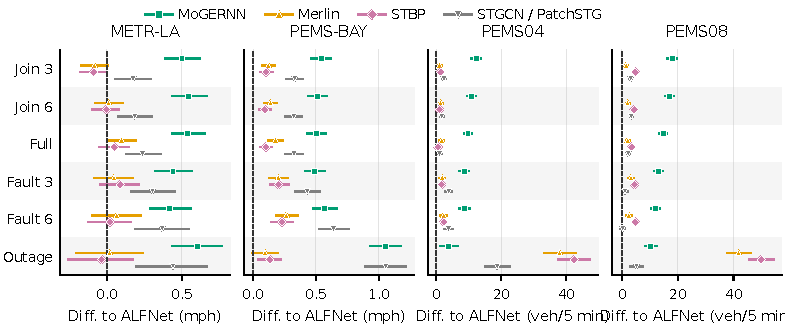
\includegraphics[width=\linewidth]{figures/figA_trajectory_diff_val.pdf}
\caption{\textbf{观测加入与中断下的配对 MAE 之差（验证集，种子32）。}横轴为比较方法减 ALFNet 的 MAE 之差，正值表示 ALFNet 更低；点为全部窗口的均值，线段为配对自助法95\%区间。Join 3、Join 6 为只保留最近3步或6步读数，Full 为完整历史，Fault 3、Fault 6、Outage 为删除最近3步、6步或全部读数。}
\label{fig:app-traj-diff}
\end{figure}

\subsection{OS 路由权重}\label{sec:B_2}

ALFGraph 的路由器把 OS 表示线性映射为五个传播专家的权重（softmax，无偏置项），因此权重是观测状态的确定函数，可以直接由训练后的参数计算，不依赖输入数据。图\ref{fig:app-router}对四个数据集、三个种子的最终模型，计算四种观测角色下的专家权重，并对图核心内的全部路由器取平均；NEW 与 OFF 另对12个状态进度取值取平均。权重随观测角色变化：与 ON 相比，各角色、各专家的平均权重最多相差0.19（均匀分配时每个专家为0.20）。例如在 PEMS-BAY 上，NEW 的自身传播（identity）权重为0.42，ON 为0.23，UNO 为0.20。可见，路由器为不同的观测角色学到了不同的专家组合。在同一角色内，状态进度从1/12变到1时，任一专家权重的变化不超过0.028，路由权重主要由角色与观测掩码决定。

\begin{figure}[tp]
\centering
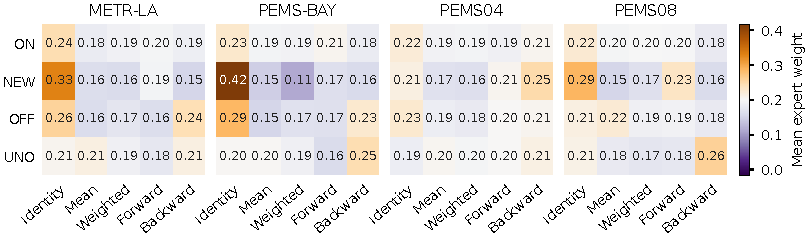
\includegraphics[width=\linewidth]{figures/figA1_router_gates.pdf}
\caption{\textbf{不同观测角色下 OS 路由器分配给五个传播专家的平均权重。}四个数据集，三个种子的均值；NEW 与 OFF 对12个状态进度取值取平均。由最终模型参数直接计算，不涉及测试数据。}
\label{fig:app-router}
\end{figure}
